
% !TeX program = xelatex
%─────────────────────────────────────────────────────────────────────────────
%  test_summary.tex
%  Beamer slide deck – MovieLens 10-fold experiment report
%─────────────────────────────────────────────────────────────────────────────
\documentclass[aspectratio=169,10pt]{beamer}

%─── 폰트 & 한국어 ───────────────────────────────────────────────────────────
\usepackage{fontspec}
\usepackage[hangul]{kotex}
\setmonofont{Consolas}

%─── 테마 ────────────────────────────────────────────────────────────────────
\usetheme{Madrid}
\usecolortheme{seahorse}
\usefonttheme[onlymath]{serif}
\setbeamertemplate{navigation symbols}{}
\setbeamertemplate{footline}{
	\leavevmode%
	\hbox{%
		\begin{beamercolorbox}[wd=.40\paperwidth,ht=2.25ex,dp=1ex,center]{author in head/foot}%
			\usebeamerfont{author in head/foot}\insertshortauthor
		\end{beamercolorbox}%
		\begin{beamercolorbox}[wd=.40\paperwidth,ht=2.25ex,dp=1ex,center]{title in head/foot}%
			\usebeamerfont{title in head/foot}\insertshorttitle
		\end{beamercolorbox}%
		\begin{beamercolorbox}[wd=.20\paperwidth,ht=2.25ex,dp=1ex,right]{date in head/foot}%
			\usebeamerfont{date in head/foot}
			\insertframenumber{} / \inserttotalframenumber\hspace*{2ex}
		\end{beamercolorbox}}%
	\vskip0pt%
}

%─── 패키지 ──────────────────────────────────────────────────────────────────
\usepackage{amsmath,amssymb,bm}
\usepackage{booktabs}
\usepackage{multirow}
\usepackage{colortbl}
\usepackage{xcolor}
\usepackage{tikz}
\usetikzlibrary{positioning,arrows,decorations.pathreplacing}
\usepackage{graphicx}

%─── 색 정의 ─────────────────────────────────────────────────────────────────
\definecolor{posblue}{RGB}{30,100,200}
\definecolor{negred}{RGB}{210,40,40}
\definecolor{testgreen}{RGB}{0,150,80}
\definecolor{hilight}{RGB}{255,230,100}

%─── 메타정보 ─────────────────────────────────────────────────────────────────
\title[MovieLens 10-Fold Report]{MovieLens 10-Fold 실험 결과 리포트\\
			 \small Baseline(\(\alpha=1\)) vs \(\alpha\)-최적화/정규화 비교}
\subtitle{랩미팅 보고용 상세 요약}
\author[발표자]{[]}
\institute{[]}
\date{\today}

\begin{document}

%─────────────────────────────────────────────────────────────────────────────
\begin{frame}
	\titlepage
\end{frame}

\begin{frame}{목차}
	\tableofcontents[hideallsubsections]
\end{frame}

%═════════════════════════════════════════════════════════════════════════════
\section{실험 목적과 설정}
%═════════════════════════════════════════════════════════════════════════════

\begin{frame}{핵심 질문}
	\begin{block}{Research Question}
		Validation 기반 \(\alpha\) 최적화(및 \(\lambda\)-정규화)가\\
		실제 Test 성능(RMSE)을 개선하는가?
	\end{block}

	\vspace{0.4em}
	\begin{columns}[T]
		\column{0.49\textwidth}
			\textbf{비교 대상}
			\begin{itemize}
				\item Baseline: \(\alpha = 1\)
				\item Optimized: Validation MSE 최소 \(\alpha\)
				\item Regularized: \(\text{MSE}_{val}+\lambda|\alpha-1|\)
			\end{itemize}

			\textbf{데이터/프로토콜}
			\begin{itemize}
				\item MovieLens 1M
				\item 10-Fold Cross Validation
				\item 17개 유사도 지표, 다양한 \(K\), TopN
			\end{itemize}

		\column{0.49\textwidth}
			\textbf{평가 지표}
			\begin{itemize}
				\item 1차: Test RMSE
				\item 보조: MAD, Precision@N, Recall@N
			\end{itemize}

			\vspace{0.4em}
			\begin{alertblock}{검증 관점}
				Validation 최적화 성과와 Test 일반화 성과를 분리해 해석.
			\end{alertblock}
	\end{columns}
\end{frame}

\begin{frame}[shrink=15]{평가 파이프라인 (요약)}
	\begin{center}
	\begin{tikzpicture}[
		box/.style={draw, rounded corners=3pt, minimum width=3.0cm,
								minimum height=0.7cm, align=center, font=\scriptsize, fill=blue!10},
		databox/.style={draw, rounded corners=2pt, minimum width=2.2cm,
								minimum height=0.45cm, align=center, font=\scriptsize, fill=gray!10},
		result/.style={box, fill=green!12},
		arrow/.style={->, thick},
		datalabel/.style={font=\tiny, text=posblue},
	]
		% 상단: 데이터 분할 설명
		\node[databox] (split) {Fold 분할};
		\node[databox, right=0.2cm of split] (inner) {Train Inner (80\%)};
		\node[databox, right=0.1cm of inner] (val) {Val (10\%)};
		\node[databox, right=0.1cm of val] (test) {Test (10\%)};

		% 중첩 표시
		\draw[decorate, decoration={brace, amplitude=3pt, mirror}, thick, gray]
			(inner.south west) -- (val.south east)
			node[midway, below=4pt, font=\tiny, text=gray] {Train Full = Inner + Val};

		% Phase 1
		\node[box, below=1.2cm of split.south west, anchor=north west] (p1)
			{Phase 1: \(\alpha\) 탐색\\{\tiny Train Inner로 예측, Val로 평가}};
		\node[datalabel, above=0.1cm of p1] {\textbf{sim\_inner} 유사도 사용};
		\node[font=\tiny, text=negred, below=0.1cm of p1]
			{$\alpha^* = \arg\min\bigl[\text{MSE}_{val} + \lambda|\alpha{-}1|\bigr]$};

		% Phase 2
		\node[box, right=1.5cm of p1] (p2)
			{Phase 2: Test 예측 생성\\{\tiny Train Full 평점 + \(\alpha^*\)로 KNN 예측}};
		\node[datalabel, above=0.1cm of p2] {\textbf{sim\_inner} 유사도 재사용};

		% Test 평가
		\node[result, below=0.8cm of p2] (eval)
			{Test 평가\\{\tiny 예측값 vs 실제값 → RMSE}};

		% 화살표
		\draw[arrow] (split) -- (inner);
		\draw[arrow] (inner) -- (val);
		\draw[arrow] (val) -- (test);
		\draw[arrow] (inner.south) -- (p1.north -| inner.south);
		\draw[arrow] (p1) -- node[above, font=\tiny]{$\alpha^*(\lambda)$} (p2);
		\draw[arrow] (p2) -- node[right, font=\tiny]{예측값} (eval);
		\draw[arrow, dashed, gray] (test.south) |- (eval.east)
			node[pos=0.25, right, font=\tiny, text=gray]{실제값};
	\end{tikzpicture}
	\end{center}

	\vspace{0.1em}
	{\small
	\begin{itemize}
		\item \textbf{Train Full} = Train Inner + Validation (Phase 2의 평점 참조용)
		\item Phase 1에서 \(\lambda\)에 따라 다른 \(\alpha^*\)가 선택됨
		\item Phase 2는 선택된 \(\alpha^*\)와 Train Full 평점으로 Test 셀의 예측값 생성
		\item Test 평가: Phase 2의 예측값과 실제 Test 평점을 비교 → RMSE/MAD/Precision
	\end{itemize}
	}
\end{frame}


%═════════════════════════════════════════════════════════════════════════════
\section{Fold·유사도 분해 분석}
%═════════════════════════════════════════════════════════════════════════════

\begin{frame}[shrink=5]{유사도(method)별 분해: 전 method에서 최적화 개선 \textnormal{\small(V6 inner\_sim, $\lambda=0.002$)}}
	\begin{columns}[T]
		\column{0.50\textwidth}
			\textbf{큰 개선 (Top 5)}
			\renewcommand{\arraystretch}{1.2}
			\begin{tabular}{l|c|c}
				\toprule
				Method & \(\Delta\)RMSE\% & Win-rate \\
				\midrule
				acos      & $-2.47\%$ & 100\% \\
				ari       & $-1.91\%$ & 100\% \\
				ami       & $-1.56\%$ & 100\% \\
				msd       & $-0.63\%$ & 78\% \\
				manhattan & $-0.56\%$ & 100\% \\
				\bottomrule
			\end{tabular}

		\column{0.48\textwidth}
			\textbf{소폭 개선 (Bottom 5)}
			\renewcommand{\arraystretch}{1.2}
			\begin{tabular}{l|c|c}
				\toprule
				Method & \(\Delta\)RMSE\% & Win-rate \\
				\midrule
				spcc    & $-0.04\%$ & 74\% \\
				cosine  & $-0.04\%$ & 50\% \\
				cpcc    & $-0.02\%$ & 66\% \\
				jaccard & $-0.01\%$ & 34\% \\
				\midrule
				\textbf{전체 평균} & $\mathbf{-0.50\%}$ & \textbf{78.9\%} \\
				\bottomrule
			\end{tabular}
	\end{columns}

	\vspace{0.4em}
	\begin{exampleblock}{핵심 변화: V5 대비 완전 역전}
		V5에서 악화되었던 euclidean($+8.97\%$), chebyshev($+8.64\%$), manhattan($+5.20\%$)이
		V6에서 각각 $-0.06\%$, $-0.12\%$, $-0.56\%$로 \textbf{전부 개선}으로 전환.
		\textbf{17개 method 전원 $\Delta \leq 0$} --- 악화 method 없음.
	\end{exampleblock}
\end{frame}

\begin{frame}[shrink=5]{하이퍼파라미터(K, TopN)별 영향 분석}
	\begin{columns}[T]
		\column{0.50\textwidth}
			\textbf{K (이웃 수)의 영향}
			\renewcommand{\arraystretch}{1.2}
			\begin{tabular}{c|c|c|c}
				\toprule
				K & Base RMSE & Opt RMSE & \(\Delta\) \\
				\midrule
				10  & 1.040 & 1.045 & +0.005 \\
				30  & 1.012 & 1.030 & +0.017 \\
				50  & \textbf{1.010} & 1.031 & +0.021 \\
				70  & 1.011 & 1.033 & +0.022 \\
				100 & 1.012 & 1.035 & +0.023 \\
				\bottomrule
			\end{tabular}
			\begin{itemize}
				\item K=50 부근에서 Baseline 성능 최고.
				\item K가 커질수록 최적화(\(\alpha\)) 적용 시 성능 악화 폭(\(\Delta\))이 더 커짐.
			\end{itemize}

		\column{0.48\textwidth}
			\textbf{TopN (추천 목록 크기)의 영향}
			\renewcommand{\arraystretch}{1.2}
			\begin{tabular}{c|c|c|c}
				\toprule
				TopN & Base RMSE & Opt RMSE & \(\Delta\) \\
				\midrule
				5  & 1.015 & 1.034 & +0.018 \\
				20 & 1.015 & 1.034 & +0.018 \\
				50 & 1.015 & 1.034 & +0.018 \\
				\bottomrule
			\end{tabular}
			\begin{itemize}
				\item TopN은 \textbf{RMSE/MAD 예측 성능에 전혀 영향을 주지 않음}.
				\item 예측 로직은 K에만 의존하며, TopN은 Precision/Recall 등 랭킹 평가 지표 계산에만 사용됨.
			\end{itemize}
	\end{columns}
\end{frame}

\begin{frame}{종합 논리: 왜 평균 결론이 baseline 우위인가?}
	\begin{enumerate}
		\item \textbf{Fold 축}: 1--10 대부분에서 optimized가 열세 (일관성)
		\item \textbf{Method 축}: 개선군보다 악화군의 폭이 더 큼 (비대칭)
		\item \textbf{Aggregation}: 전체 조합 평균 시 열세가 누적
	\end{enumerate}

	\vspace{0.4em}
	\begin{block}{실무적 해석}
		\(\alpha\)-최적화는 ``항상 적용''보다
		\textbf{method 선택적 적용}이 더 타당하며,
		기본 정책은 \(\alpha=1\) baseline이 안전.
	\end{block}
\end{frame}

%═════════════════════════════════════════════════════════════════════════════
\section{원인 분석}
%═════════════════════════════════════════════════════════════════════════════

\begin{frame}{왜 과적합이 발생하는가?}
	\begin{block}{관측된 메커니즘}
		\begin{enumerate}
			\item Validation에서 \(\alpha\neq1\)가 MSE를 낮춤
			\item 선택된 \(\alpha\)를 Test에 적용하면 성능 저하 빈번
			\item Validation 분포가 Test 일반화를 충분히 대표하지 못함
		\end{enumerate}
	\end{block}

	\vspace{0.3em}
	\begin{columns}[T]
		\column{0.48\textwidth}
			\textbf{근거 A: 구성별 혼합 성능}
			\begin{itemize}
				\item (1--10 fold 평균) optimized: +1.41\% 악화
				\item fold별 차이는 대부분 양수(예외: fold5는 +0.03\%)
			\end{itemize}

			\textbf{근거 B: 방법별 편차}
			\begin{itemize}
				\item ACOS: -2.51\% (개선)
				\item EUCLIDEAN: +8.97\% (악화)
			\end{itemize}

		\column{0.48\textwidth}
			\textbf{근거 C: 단순 모델의 안정성}
			\begin{itemize}
				\item \(\alpha=1\): 조합 간 분산이 작고 일관
				\item 최적화 \(\alpha\): 조합별 값이 달라 변동성 증가
			\end{itemize}

			\begin{alertblock}{요약}
				Validation 최적화 신호가 Test 일반화 신호와 불일치.
			\end{alertblock}
	\end{columns}
\end{frame}

\begin{frame}[shrink=5]{시각화 기반 구체적 패턴 분석 (Validation vs Test)}
	\begin{columns}[T]
		\column{0.48\textwidth}
			\textbf{Validation vs Test 개선도 산점도}
			\begin{center}
				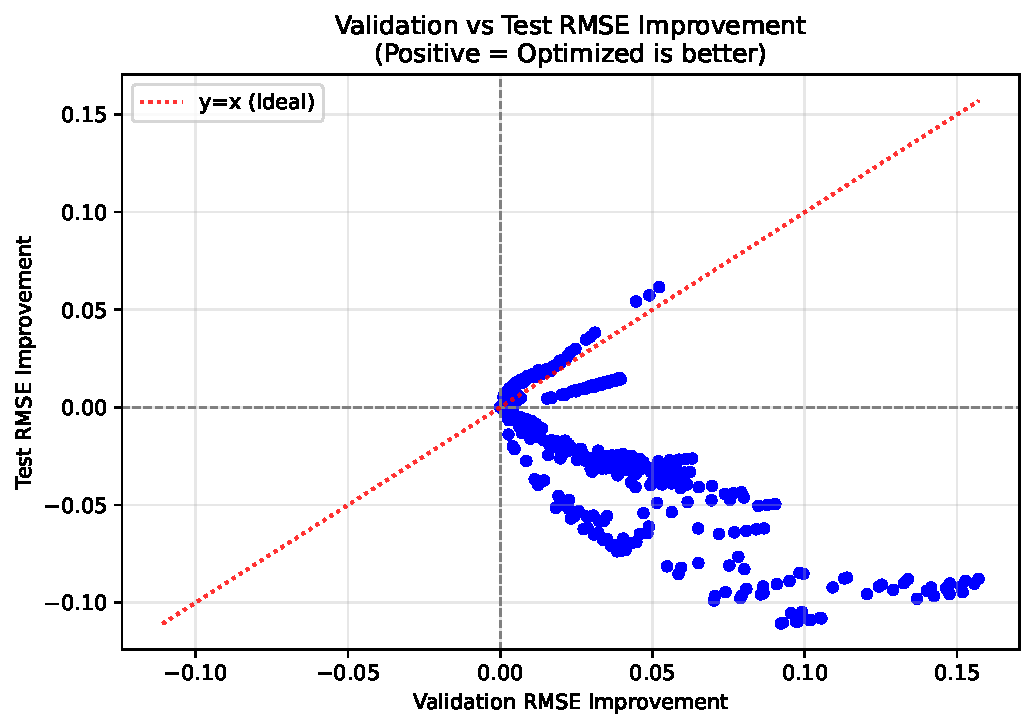
\includegraphics[width=0.95\textwidth]{../results/figures/val_vs_test_scatter.pdf}
			\end{center}
			{\scriptsize * 양수(+)는 Optimized가 Baseline보다 우수함을 의미}

		\column{0.50\textwidth}
			\textbf{과적합(Overfitting) 패턴 확인}
			\begin{itemize}
				\item \textbf{Validation}: 대부분의 점이 0보다 큼 (우측 분포).
				\item \textbf{Test}: 대부분의 점이 0보다 작음 (하단 분포).
				\item 즉, Validation에서의 성능 향상이 Test로 이어지지 않음.
			\end{itemize}

			\vspace{0.3em}
			\textbf{유사도별 구체적 편차 (Test RMSE 개선도)}
			\renewcommand{\arraystretch}{1.2}
			\begin{tabular}{l|c|c}
				\toprule
				Method & \(\Delta\) Test RMSE\% & 평가 \\
				\midrule
				\texttt{acos} & $-2.51\%$ & 개선 (우수) \\
				\texttt{msd}  & $-0.95\%$ & 개선 (우수) \\
				\texttt{pcc}  & $+3.03\%$ & 악화 (열세) \\
				\texttt{euclidean} & $+8.97\%$ & 크게 악화 \\
				\bottomrule
			\end{tabular}
			{\scriptsize $\Delta = (\text{RMSE}_{opt}-\text{RMSE}_{base})/\text{RMSE}_{base}\times100$;\\음수(−)는 Optimized 우위.}
			\begin{itemize}
				\item \(\lambda\) 값이 커질수록(정규화 강도 증가) Test에서의 성능 악화 폭이 줄어드는 경향 관찰.
			\end{itemize}
	\end{columns}
\end{frame}

\begin{frame}{\(\lambda\)와 \(\alpha\) 분포 변화 (\texttt{lambda\_validation\_simulation.csv})}
	\begin{center}
	\renewcommand{\arraystretch}{1.25}
	\begin{tabular}{c|c|c|c}
		\toprule
		\(\lambda\) & Avg \(\alpha\) & Extreme \(\alpha\ge2\) & Near baseline (0.9--1.1) \\
		\midrule
		0.000 & 3.852 & 69.8\% & 1.1\% \\
		0.010 & 2.252 & 42.7\% & 32.8\% \\
		0.020 & 1.843 & 37.5\% & 42.6\% \\
		0.030 & 1.563 & 30.0\% & 51.8\% \\
		0.050 & 1.127 & 5.8\%  & 77.4\% \\
		0.100 & 0.995 & 0.0\%  & 98.6\% \\
		\bottomrule
	\end{tabular}
	\end{center}

	\vspace{0.4em}
	\begin{itemize}
		\item \(\lambda\uparrow\)는 분명히 extreme \(\alpha\)를 줄임
		\item 하지만 최종 RMSE 관점에서는 \(\alpha=1\) 단순 baseline이 여전히 최강
	\end{itemize}
\end{frame}

\begin{frame}[shrink=5]{시각 자료: \(\lambda\) 시뮬레이션 분석}
	\begin{center}
		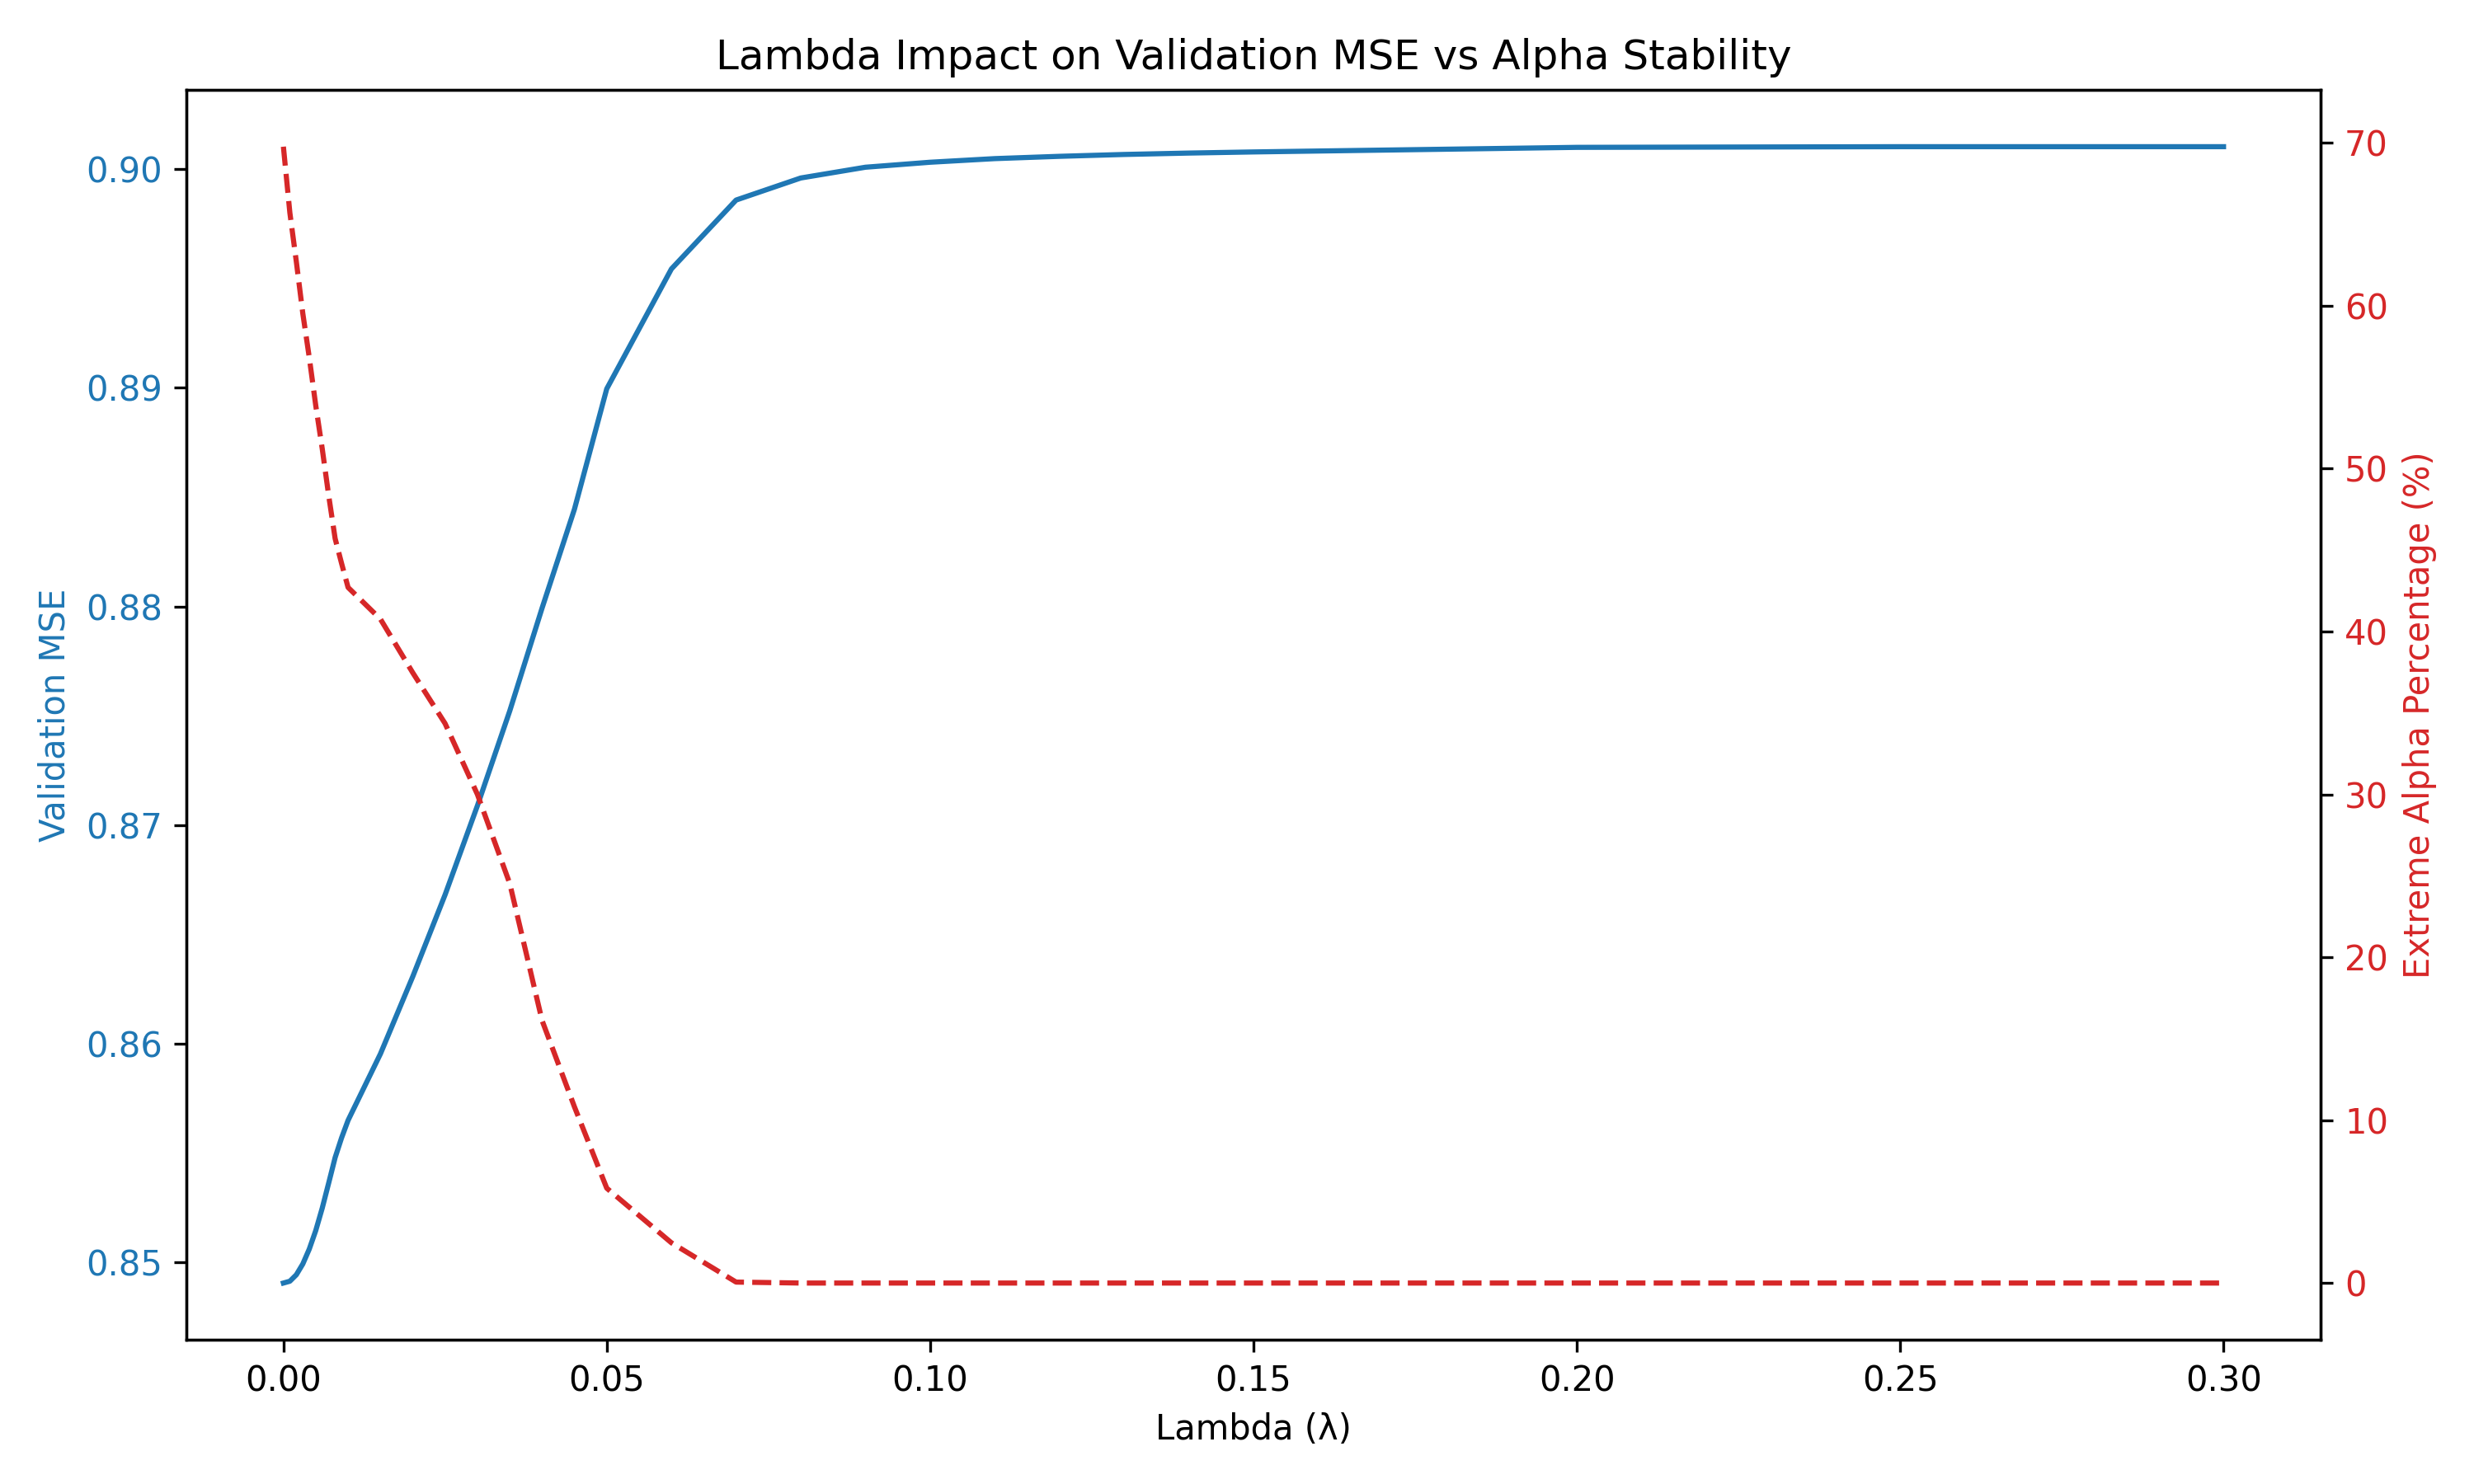
\includegraphics[width=0.86\textwidth]{../results/lambda_optimization/lambda_validation_analysis.png}
	\end{center}
	\vspace{0.2em}
	{\small
	그림은 \(\lambda\) 증가 시 분포 안정화 경향을 보여주며,
	실제 운영 선택에서는 ``안정화 효과 vs baseline 성능''의 trade-off를 함께 봐야 함.
	}
\end{frame}

%═════════════════════════════════════════════════════════════════════════════
\section{실무 권고안}
%═════════════════════════════════════════════════════════════════════════════

\begin{frame}{의사결정 가이드}
	\renewcommand{\arraystretch}{1.3}
	\begin{tabular}{l|l|l}
		\toprule
		\textbf{목표} & \textbf{권장 설정} & \textbf{이유} \\
		\midrule
		최고 RMSE 성능 & \textbf{\(\alpha=1\) 고정} & Test RMSE 최소 \\
		재현성/해석성 & \(\alpha=1\) 고정 & 파라미터 단순, 설명 용이 \\
		안정성 중심 완화안 & \(\lambda\in[0.02,0.03]\) & extreme \(\alpha\) 감소 \\
		method별 미세 튜닝 & method별 정책 분리 & ACOS/ARI와 EUCLIDEAN 이질성 \\
		\bottomrule
	\end{tabular}

	\vspace{0.5em}
	\begin{alertblock}{현재 프로젝트 기본안}
		운영 기본값은 \textbf{\(\alpha=1\)}를 채택하고,
		method별 후속 실험에서만 제한적으로 \(\lambda\)-정규화 적용.
	\end{alertblock}
\end{frame}

\begin{frame}{후속 실험 제안 (Conference-ready)}
	\begin{enumerate}
		\item \textbf{Method-specific regularization}: 17개 method에 개별 \(\lambda\) 매핑
		\item \textbf{완전 10-fold 재검증}: 동일 파이프라인으로 fold별 분산 보고
		\item \textbf{목적함수 확장}: RMSE 외 Precision@N 중심 최적화 비교
		\item \textbf{정책형 결론}: 
			\begin{itemize}
				\item 기본 정책: \(\alpha=1\)
				\item 예외 정책: 일부 method만 최적 \(\alpha\) 사용
			\end{itemize}
	\end{enumerate}

	\vspace{0.4em}
	\begin{block}{발표 메시지}
		``복잡한 최적화보다, \(\alpha=1\) baseline의 강건성이 실제 Test에서 더 우수했다.''
	\end{block}
\end{frame}

\begin{frame}[plain]
	\begin{center}
		\vspace{2.0cm}
		{\LARGE 감사합니다}\\[1.2em]
		{\large 질문 및 토론 환영합니다}\\[2em]
		\begin{tabular}{ll}
			\textbf{슬라이드} & \texttt{documentation/test\_summary.tex} \\
			\textbf{핵심 결과} & \texttt{results/lambda\_comprehensive\_analysis\_corrected\_20260123\_120312.csv} \\
			\textbf{분석 노트} & \texttt{docs/LAMBDA\_ANALYSIS\_SUMMARY.md}
		\end{tabular}
	\end{center}
\end{frame}

%═════════════════════════════════════════════════════════════════════════════
\section{Claude 분석: 10-Fold 전체 재검토}
%═════════════════════════════════════════════════════════════════════════════

%── 책갈피 슬라이드 ──────────────────────────────────────────────────────────
\begin{frame}[plain]
	\begin{center}
		\vspace{2.2cm}
		{\LARGE \textbf{Claude 분석}}\\[0.8em]
		{\large 10-Fold 전체 결과 재검토 및 메커니즘 분석}\\[0.6em]
		{\small fold 8--10 집계 → \textbf{전체 10-fold} (N=17,000 configs)로 확장}
	\end{center}
\end{frame}

%── 슬라이드 1: 전체 요약 ─────────────────────────────────────────────────────
\begin{frame}{10-Fold 전체 요약: 결론은 동일, 수치 갱신}
	\begin{center}
	\renewcommand{\arraystretch}{1.35}
	\begin{tabular}{l|c|c|c}
		\toprule
		\textbf{설정} & \textbf{Test RMSE} & \textbf{vs Baseline} & \textbf{Win Rate} \\
		\midrule
		\rowcolor{testgreen!20}
		\textbf{Baseline (\(\alpha=1\))} & \textbf{1.010179} & \textbf{기준} & -- \\
		Optimized (전체 평균) & 1.024460 & $+1.43\%$ \textcolor{negred}{$\uparrow$} & 31.6\% \\
		\bottomrule
	\end{tabular}
	\end{center}

	\vspace{0.4em}
	\begin{columns}[T]
		\column{0.50\textwidth}
			\textbf{이전 집계(fold 8--10)와 비교}
			\begin{itemize}
				\item 이전: $\Delta=+1.87\%$, Win=20.6\%
				\item 현재(전체): $\Delta=+1.43\%$, Win=31.6\%
				\item \(\to\) 초기 fold(1--7)에서 overfitting이 다소 완화
			\end{itemize}
		\column{0.46\textwidth}
			\begin{alertblock}{결론 유지}
				10-fold 전체로 확장해도\\
				\(\alpha=1\) baseline 우위는 불변.
			\end{alertblock}
	\end{columns}
\end{frame}

%── 슬라이드 2: Fold별 결과 ───────────────────────────────────────────────────
\begin{frame}[shrink=5]{Fold별 결과: 전체 10-Fold (갱신)}
	\begin{columns}[T]
		\column{0.48\textwidth}
		\renewcommand{\arraystretch}{1.2}
		\begin{tabular}{c|c|c|c}
			\toprule
			Fold & Base & Opt & \(\Delta\%\) \\
			\midrule
			1 & 1.0072 & 1.0197 & $+1.26$ \\
			2 & 1.0058 & 1.0165 & $+1.07$ \\
			3 & 1.0133 & 1.0254 & $+1.21$ \\
			4 & 1.0135 & 1.0270 & $+1.35$ \\
			5 & 0.9970 & 0.9973 & $+0.04$ \\
			\bottomrule
		\end{tabular}

		\column{0.48\textwidth}
		\renewcommand{\arraystretch}{1.2}
		\begin{tabular}{c|c|c|c}
			\toprule
			Fold & Base & Opt & \(\Delta\%\) \\
			\midrule
			6  & 1.0098 & 1.0270 & $+1.73$ \\
			7  & 1.0098 & 1.0296 & $+1.98$ \\
			8  & 1.0274 & 1.0448 & $+1.71$ \\
			9  & 1.0060 & 1.0264 & $+2.05$ \\
			10 & 1.0120 & 1.0310 & $+1.89$ \\
			\bottomrule
		\end{tabular}
	\end{columns}

	\vspace{0.3em}
	\begin{itemize}
		\item \textbf{10-fold 평균}: Baseline 1.0102 vs Optimized 1.0244 ($\Delta=+1.43\%$)
		\item Fold~5(+0.04\%)를 제외한 9개 fold 모두 최적화가 열세
		\item \textbf{fold 9가 최대 악화}($+2.05\%$), fold 5가 사실상 동률
	\end{itemize}
	{\scriptsize 집계: 17개 유사도 × K(10--100) × TopN(5--50) 평균}
\end{frame}

%── 슬라이드 3: Method 분류 ───────────────────────────────────────────────────
\begin{frame}[shrink=5]{Method별 분류: 최적화 효과의 이질성 (10-fold)}
	\begin{columns}[T]
		\column{0.49\textwidth}
			\textbf{\textcolor{testgreen}{Group A}: 최적화 일관 개선}
			\renewcommand{\arraystretch}{1.15}
			\begin{tabular}{l|r|r}
				\toprule
				Method & $\Delta\%$ & Win \\
				\midrule
				\texttt{acos} & $-2.54$ & 100\% \\
				\texttt{ari}  & $-1.03$ & 93\% \\
				\texttt{ami}  & $-0.72$ & 91\% \\
				\bottomrule
			\end{tabular}
			{\scriptsize 모두 $\bar\alpha<1$: 유사도 차이 \textbf{완화}}

			\vspace{0.6em}
			\textbf{\textcolor{posblue}{Group B}: 미미/혼재}
			\renewcommand{\arraystretch}{1.15}
			\begin{tabular}{l|r|r}
				\toprule
				Method & $\Delta\%$ & Win \\
				\midrule
				\texttt{msd}     & $-0.48$ & 58\% \\
				\texttt{jmsd}    & $-0.12$ & 60\% \\
				\texttt{ipwr}    & $-0.08$ & 59\% \\
				\texttt{cosine}  & $-0.06$ & 37\% \\
				\texttt{jaccard} & $-0.01$ & 26\% \\
				\bottomrule
			\end{tabular}

		\column{0.49\textwidth}
			\textbf{\textcolor{negred}{Group C}: 최적화 일관 악화}
			\renewcommand{\arraystretch}{1.15}
			\begin{tabular}{l|r|r}
				\toprule
				Method & $\Delta\%$ & Win \\
				\midrule
				\texttt{itr}           & $+0.19$ & 3\% \\
				\texttt{src}           & $+1.57$ & 1\% \\
				\texttt{kendall\_tau\_b}& $+1.75$ & 0\% \\
				\texttt{spcc}          & $+1.97$ & 0\% \\
				\texttt{pcc}           & $+2.27$ & 1\% \\
				\texttt{cpcc}          & $+2.98$ & 5\% \\
				\texttt{manhattan}     & $+4.39$ & 0\% \\
				\texttt{chebyshev}     & $+6.87$ & 2\% \\
				\texttt{euclidean}     & $+7.34$ & 1\% \\
				\bottomrule
			\end{tabular}
			{\scriptsize 모두 $\bar\alpha\gg1$: 유사도 차이 \textbf{증폭} → Overfitting}
	\end{columns}
\end{frame}

%── 슬라이드 4: 메커니즘 분석 ─────────────────────────────────────────────────
\begin{frame}{메커니즘 분석: \(\alpha\)의 두 가지 역할}
	\begin{block}{핵심 관찰}
		$S^{\alpha}$에서 \(\alpha\)는 유사도 차이를 \textbf{완화}(\(\alpha<1\)) 또는
		\textbf{증폭}(\(\alpha>1\))하는 두 가지 반대 방향으로 작용.
	\end{block}

	\vspace{0.3em}
	\begin{columns}[T]
		\column{0.48\textwidth}
			\textbf{Group A: \(\alpha<1\) = Smoothing}
			\begin{itemize}
				\item 이웃 간 가중치 차이를 줄임
				\item 더 많은 이웃을 균등하게 참고
				\item \(\to\) 정규화 효과 → 일반화 개선
			\end{itemize}
			\vspace{0.3em}
			\begin{exampleblock}{직관}
				``작은 유사도 차이에 덜 민감하게
				만들어 robust한 예측 달성''
			\end{exampleblock}

		\column{0.48\textwidth}
			\textbf{Group C: \(\alpha\gg1\) = Sharpening}
			\begin{itemize}
				\item 극소수의 아주 유사한 이웃에 집중
				\item Validation의 특정 분포에 과적합
				\item \(\to\) Test에서 일반화 실패
			\end{itemize}
			\vspace{0.3em}
			\begin{alertblock}{직관}
				``Validation의 우연한 패턴을
				학습 → Test에서 과적합 발현''
			\end{alertblock}
	\end{columns}

	\vspace{0.3em}
	\begin{center}
		\textbf{Validation 최고 RMSE} \(\neq\) \textbf{Test 최고 RMSE}: 두 값의 불일치가 핵심 문제.
	\end{center}
\end{frame}

%── 슬라이드 5: 전략적 시사점 ─────────────────────────────────────────────────
\begin{frame}{전략적 시사점 및 후속 방향}
	\begin{columns}[T]
		\column{0.50\textwidth}
			\textbf{현재 결과의 의미}
			\begin{itemize}
				\item ``\(\alpha\) 최적화 무효''가 아니라
					\textbf{method-dependent}한 것이 핵심 발견
				\item Group A의 smoothing 효과는 재현 가능한 개선
				\item 이 자체가 논문의 contribution 가능
			\end{itemize}

		\column{0.46\textwidth}
			\textbf{후속 실험 (우선순위)}
			\begin{enumerate}
				\item \textbf{Method-selective 정책} 검증:\\
					Group A: optimal \(\alpha\) 사용\\
					Group C: \(\alpha=1\) 고정\\
					→ 전체 hybrid RMSE 계산
				\item \(\alpha\) 범위를 \([0,2]\)로 제한 후\\
					Group C 과적합 감소 확인
				\item Nested CV로 validation\\
					overfitting 정도 정량화
			\end{enumerate}
	\end{columns}

	\vspace{0.4em}
	\begin{block}{발표 가능한 메시지}
		``유사도 함수의 특성에 따라 \(\alpha\) 최적화 효과가 결정된다.
		\(\alpha<1\)(smoothing)은 일반화를 개선하고,
		\(\alpha\gg1\)(sharpening)은 validation overfitting을 유발한다.''
	\end{block}
\end{frame}

%═════════════════════════════════════════════════════════════════════════════
\section{파이프라인 점검: 잠재적 이슈 2가지}
%═════════════════════════════════════════════════════════════════════════════

%── 책갈피 ────────────────────────────────────────────────────────────────────
\begin{frame}[plain]
	\begin{center}
		\vspace{2.2cm}
		{\LARGE \textbf{파이프라인 점검}}\\[0.8em]
		{\large 유사도 계산 데이터 소스 \& 음수 클리핑 영향}
	\end{center}
\end{frame}

%── 이슈 1: 유사도 데이터 소스 ────────────────────────────────────────────────
\begin{frame}{이슈 1: 유사도 행렬이 train\_full로 계산됨}
	\begin{alertblock}{발견 사항}
		\texttt{sim\_*.npy}는 \texttt{train.csv} (train\_inner + validation, 90\%)로
		사전 계산됨. Phase~1에서 validation 데이터가 유사도에 이미 반영.
	\end{alertblock}

	\vspace{0.3em}
	\begin{center}
	\begin{tikzpicture}[
		box/.style={draw, rounded corners=2pt, minimum width=2.4cm,
					minimum height=0.7cm, align=center, font=\small},
		leak/.style={box, fill=negred!15},
		ok/.style={box, fill=testgreen!15},
		arrow/.style={->, thick}
	]
		\node[leak] (sim) {유사도 계산\\{\scriptsize train\_full (90\%)}};
		\node[ok, right=0.8cm of sim] (p1) {Phase 1\\{\scriptsize 학습: train\_inner}};
		\node[ok, right=0.8cm of p1] (val) {평가\\{\scriptsize validation}};
		\node[ok, below=0.6cm of p1] (p2) {Phase 2\\{\scriptsize 학습: train\_full}};
		\node[ok, right=0.8cm of p2] (test) {평가\\{\scriptsize test}};

		\draw[arrow] (sim) -- (p1);
		\draw[arrow, dashed, negred] (sim) -- node[above, font=\tiny, negred]{val 포함!} (val);
		\draw[arrow] (p1) -- (val);
		\draw[arrow] (sim) -- (p2);
		\draw[arrow] (p2) -- (test);
	\end{tikzpicture}
	\end{center}

	\vspace{0.2em}
	\begin{columns}[T]
		\column{0.50\textwidth}
			\textbf{영향}
			\begin{itemize}
				\item Validation MSE가 낙관적으로 산출
				\item \(\alpha\neq1\)이 실제보다 ``좋아 보임''
				\item Test에서 이 이점 부재 → 성능 하락
			\end{itemize}
		\column{0.46\textwidth}
			\textbf{대응 방안}
			\begin{itemize}
				\item \textbf{train\_inner}로 유사도 재계산
				\item 동일 실험 재수행하여 비교
				\item 누수 제거 시 \(\alpha\) 최적화\\
					효과가 달라지는지 검증
			\end{itemize}
	\end{columns}
\end{frame}

%── 이슈 2: 음수 클리핑 ──────────────────────────────────────────────────────
\begin{frame}[shrink=5]{이슈 2: 음수 유사도 클리핑과 \(\alpha\)의 상호작용}
	\begin{block}{현재 구현}
		$S^{(\alpha)} = \max(S, 0)^{\alpha}$
		\hfill {\small 음수 → 0 \textbf{후} \(\alpha\) 승}
	\end{block}

	\vspace{0.3em}
	\begin{columns}[T]
		\column{0.48\textwidth}
			\textbf{음수 비율 (fold\_01 기준)}
			\renewcommand{\arraystretch}{1.15}
			\begin{tabular}{l|c|l}
				\toprule
				Method & 음수\% & Group \\
				\midrule
				ari   & 41.4\% & A \\
				ami   & 40.9\% & A \\
				pcc   & 30.0\% & C \\
				acos  & 29.0\% & A \\
				cosine & 0\%   & B \\
				euclidean & 0\% & C \\
				\bottomrule
			\end{tabular}

		\column{0.50\textwidth}
			\textbf{\(\alpha\)와의 상호작용}

			{\small\textbf{Group A} (\(\alpha<1\)): 이중 이득}
			\begin{itemize}\small
				\item 클리핑 → 노이즈(반상관) 제거
				\item \(\alpha<1\) → 가중치 균등화
				\item \(\to\) 정규화 효과 강화
			\end{itemize}

			\vspace{0.2em}
			{\small\textbf{Group C} (\(\alpha\gg1\)): 이중 손해}
			\begin{itemize}\small
				\item 클리핑 → 이웃 다양성 감소
				\item \(\alpha\gg1\) → 상위 1--2명에 집중
				\item K=20 요청 → \textbf{실효 K$\approx$2--3}
				\item \(\to\) 과적합 구조 형성
			\end{itemize}
	\end{columns}

	\vspace{0.3em}
	\begin{center}
	\renewcommand{\arraystretch}{1.2}
	\begin{tabular}{c|c|c|c}
		\toprule
		& 클리핑 효과 & \(\alpha\) 효과 & 합산 \\
		\midrule
		\textbf{Group A} (\(\alpha<1\)) & 노이즈 제거 (이득) & 균등화 (이득) & \textcolor{testgreen}{\textbf{이중 이득}} \\
		\textbf{Group C} (\(\alpha\gg1\)) & 다양성 손실 (손해) & 집중화 (손해) & \textcolor{negred}{\textbf{이중 손해}} \\
		\bottomrule
	\end{tabular}
	\end{center}
\end{frame}

%═════════════════════════════════════════════════════════════════════════════
\section{inner\_sim 실험: Validation 누수 제거 효과 (Fold 01)}
%═════════════════════════════════════════════════════════════════════════════

%── 책갈피 ────────────────────────────────────────────────────────────────────
\begin{frame}[plain]
	\begin{center}
		\vspace{2.2cm}
		{\LARGE \textbf{inner\_sim 실험}}\\[0.8em]
		{\large Validation 누수 제거 후 Fold 01 결과 분석}\\[0.6em]
		{\small \texttt{sim\_inner\_\{method\}.npy} (train\_inner 전용) 적용\\
		결과: \texttt{results/inner\_sim/fold\_01/} (2026-03-11)}
	\end{center}
\end{frame}

%── 슬라이드 1: 배경 및 변경 내용 ────────────────────────────────────────────
\begin{frame}{inner\_sim 실험: 무엇이 달라졌는가?}
	\begin{alertblock}{기존 파이프라인의 문제 (이슈 1 재확인)}
		\texttt{sim\_*.npy}는 \texttt{train\_full}(train\_inner + validation, 90\%)로
		계산 → Phase~1 alpha 최적화 시 validation 데이터가 유사도에 이미 반영됨.
	\end{alertblock}

	\vspace{0.4em}
	\begin{columns}[T]
		\column{0.48\textwidth}
			\textbf{기존 방식}
			\begin{itemize}
				\item 유사도: \texttt{train\_full} 기반
				\item alpha 탐색 시 val 누수 발생
				\item Validation RMSE가 낙관적으로 측정됨
			\end{itemize}

		\column{0.48\textwidth}
			\textbf{inner\_sim 방식}
			\begin{itemize}
				\item 유사도: \textbf{train\_inner 전용}으로 재계산
				\item alpha 탐색 시 val 누수 없음
				\item 공정한 validation 평가 보장
			\end{itemize}
	\end{columns}

	\vspace{0.5em}
	\begin{block}{검증 파일}
		\begin{tabular}{l|l}
			Old & \texttt{results/fold\_01/grid\_search\_results\_reeval\_lambda\_0.002\_v2.csv}\\
			New & \texttt{results/inner\_sim/fold\_01/grid\_search\_results\_20260311\_132613.csv}
		\end{tabular}
	\end{block}
\end{frame}

%── 슬라이드 2: 최적 Alpha 변화 ───────────────────────────────────────────────
\begin{frame}[shrink=30]{Alpha 최적값의 극적 변화 (K=20, TopN=20 기준)}
	\begin{center}
	\renewcommand{\arraystretch}{1.25}
	\begin{tabular}{l|c|c|c|c|c}
		\toprule
		\textbf{Method} & \textbf{Old $\alpha$} & \textbf{New $\alpha$} & \textbf{Old Val RMSE} & \textbf{New Val RMSE} & \textbf{해석} \\
		\midrule
		chebyshev    & \textcolor{negred}{7.50} & 1.00 & \textcolor{negred}{0.804} & 1.011 & 극단 과적합 제거 \\
		msd          & \textcolor{negred}{10.00}& 1.00 & \textcolor{negred}{0.824} & 0.986 & 극단 과적합 제거 \\
		cpcc         & \textcolor{negred}{7.00} & 1.00 & \textcolor{negred}{0.811} & 0.997 & 극단 과적합 제거 \\
		euclidean    & \textcolor{negred}{4.00} & 0.55 & \textcolor{negred}{0.851} & 1.018 & 과적합 제거 \\
		pcc          & \textcolor{negred}{3.50} & 0.55 & \textcolor{negred}{0.826} & 1.016 & 과적합 제거 \\
		spcc         & \textcolor{negred}{3.50} & 0.65 & \textcolor{negred}{0.827} & 1.015 & 과적합 제거 \\
		kendall\_tau\_b& \textcolor{negred}{2.50}& 0.10 & \textcolor{negred}{0.856} & 1.023 & 과적합 제거 \\
		manhattan    & \textcolor{negred}{1.75} & 0.25 & \textcolor{negred}{0.915} & 1.027 & 과적합 제거 \\
		acos         & 0.05 & 0.05 & 1.002 & 1.026 & 안정적 (변화 없음) \\
		\midrule
		\textbf{평균}& \textbf{2.86} & \textbf{0.56} & \textbf{0.913} & \textbf{1.017} & \\
		\bottomrule
	\end{tabular}
	\end{center}

	\vspace{0.3em}
	\begin{alertblock}{핵심}
		기존 방식에서 Val RMSE가 낙관적으로 측정될수록 alpha가 극단적으로 커졌음.
		inner\_sim 적용 시 alpha가 \textbf{0.56}으로 수렴 (기존 \textbf{2.86}).
	\end{alertblock}
\end{frame}

%── 슬라이드 3: 과적합 정도 비교 ─────────────────────────────────────────────
\begin{frame}{Validation–Test RMSE 갭: 과적합 정도 비교}
	\begin{center}
	\renewcommand{\arraystretch}{1.35}
	\begin{tabular}{l|c|c|c}
		\toprule
		\textbf{설정} & \textbf{Val RMSE} & \textbf{Test RMSE} & \textbf{Val–Test 갭} \\
		\midrule
		Old (train\_full 유사도) & 0.913 & 1.026 & \textcolor{negred}{+0.106 (심한 과적합)} \\
		\rowcolor{testgreen!20}
		New (inner\_sim) & 1.017 & 1.005 & \textcolor{testgreen}{-0.010 (사실상 일치)} \\
		\bottomrule
	\end{tabular}
	\end{center}

	\vspace{0.4em}
	\begin{columns}[T]
		\column{0.50\textwidth}
			\textbf{기존 방식 해석}
			\begin{itemize}
				\item Val RMSE 0.913 → 실제보다 0.113 낮게 측정
				\item alpha 최적화가 실제보다 효과적으로 보임
				\item Test에서 +0.106 갭 → 전형적 data leakage 패턴
			\end{itemize}

		\column{0.46\textwidth}
			\textbf{inner\_sim 해석}
			\begin{itemize}
				\item Val RMSE $\approx$ Test RMSE (갭: -0.01)
				\item 공정한 alpha 탐색 결과
				\item Test 성능이 Validation을 충실히 반영
			\end{itemize}
	\end{columns}
\end{frame}

%── 슬라이드 4: Method별 Test RMSE 비교 ───────────────────────────────────────
\begin{frame}[shrink=55]{Method별 Test RMSE: 공정 비교 포함 (전체 K/TopN 평균)}
	\begin{center}
	\renewcommand{\arraystretch}{1.15}
	\begin{tabular}{l|cc|c|c|cc}
		\toprule
		\multirow{2}{*}{\textbf{Method}}
		  & \multicolumn{2}{c|}{\textbf{Old (train\_full)}}
		  & \textbf{New}
		  & \textbf{Base}
		  & \multicolumn{2}{c}{\textbf{New 개선폭}} \\
		  & $\lambda{=}0.002$ & $\lambda{=}0.030^{\dagger}$
		  & \small(inner, $\lambda{=}0.002$)
		  & \small($\alpha{=}1$)
		  & vs Old$_{002}$ & vs Old$_{030}$ \\
		\midrule
		chebyshev      & 1.0923 & 1.0245 & \textcolor{testgreen}{1.0015} & 1.0024 & \textcolor{testgreen}{$-0.091$} & \textcolor{testgreen}{$-0.023$} \\
		euclidean      & 1.0915 & 1.0413 & \textcolor{testgreen}{1.0071} & 1.0077 & \textcolor{testgreen}{$-0.084$} & \textcolor{testgreen}{$-0.034$} \\
		manhattan      & 1.0657 & 1.0445 & \textcolor{testgreen}{1.0153} & 1.0214 & \textcolor{testgreen}{$-0.050$} & \textcolor{testgreen}{$-0.029$} \\
		cpcc           & 1.0257 & 0.9809 & \textcolor{testgreen}{0.9834} & 0.9836 & \textcolor{testgreen}{$-0.042$} & \textcolor{negred}{$+0.003$} \\
		pcc            & 1.0353 & 1.0088 & \textcolor{testgreen}{1.0063} & 1.0075 & \textcolor{testgreen}{$-0.029$} & \textcolor{testgreen}{$-0.003$} \\
		spcc           & 1.0292 & 1.0064 & \textcolor{testgreen}{1.0055} & 1.0061 & \textcolor{testgreen}{$-0.024$} & \textcolor{testgreen}{$-0.001$} \\
		kendall\_tau\_b& 1.0321 & 1.0120 & \textcolor{testgreen}{1.0098} & 1.0128 & \textcolor{testgreen}{$-0.022$} & \textcolor{testgreen}{$-0.002$} \\
		src            & 1.0309 & 1.0117 & \textcolor{testgreen}{1.0095} & 1.0123 & \textcolor{testgreen}{$-0.021$} & \textcolor{testgreen}{$-0.002$} \\
		itr            & 1.0317 & 1.0272 & \textcolor{testgreen}{1.0236} & 1.0271 & \textcolor{testgreen}{$-0.008$} & \textcolor{testgreen}{$-0.004$} \\
		ami            & 1.0241 & 1.0312 & 1.0260 & 1.0412 & \textcolor{negred}{$+0.002$} & \textcolor{testgreen}{$-0.005$} \\
		ari            & 1.0209 & 1.0275 & 1.0241 & 1.0434 & \textcolor{negred}{$+0.003$} & \textcolor{testgreen}{$-0.003$} \\
		acos           & 1.0126 & 1.0158 & 1.0114 & 1.0405 & \textcolor{testgreen}{$-0.001$} & \textcolor{testgreen}{$-0.004$} \\
		jmsd           & 0.9993 & 1.0019 & 1.0011 & 1.0029 & \textcolor{negred}{$+0.002$} & \textcolor{testgreen}{$-0.001$} \\
		msd            & \textcolor{testgreen}{0.9695} & 0.9786 & 0.9760 & 0.9831 & \textcolor{negred}{$+0.007$} & \textcolor{testgreen}{$-0.003$} \\
		ipwr           & \textcolor{testgreen}{0.9625} & 0.9641 & 0.9633 & 0.9646 & \textcolor{negred}{$+0.001$} & \textcolor{testgreen}{$-0.001$} \\
		cosine         & 1.0037 & 1.0051 & 1.0061 & 1.0068 & \textcolor{negred}{$+0.002$} & \textcolor{negred}{$+0.001$} \\
		jaccard        & 1.0096 & 1.0100 & 1.0110 & 1.0113 & \textcolor{negred}{$+0.001$} & \textcolor{negred}{$+0.001$} \\
		\midrule
		\textbf{평균}  & 1.0257 & 1.0113 & \textbf{1.0048} & 1.0103
		  & \textcolor{testgreen}{$\mathbf{-0.021}$} & \textcolor{testgreen}{$\mathbf{-0.007}$} \\
		\bottomrule
	\end{tabular}
	\end{center}
	{\scriptsize $\dagger$ Old($\lambda{=}0.030$)은 기존 방식에서의 최선 lambda. 개선: vs Old$_{002}$는 9/17, vs Old$_{030}$는 15/17.}
\end{frame}

%── 슬라이드 4-1: Lambda별 비교 보정 ─────────────────────────────────────────
\begin{frame}[shrink=15]{Lambda별 Test RMSE: 대표값 선정 근거}
	\begin{columns}[T]
		\column{0.50\textwidth}
			\begin{center}
			\renewcommand{\arraystretch}{1.1}
			\begin{tabular}{l|r|r|c}
				\toprule
				\textbf{설정} & \textbf{avg $\alpha$} & \textbf{RMSE} & \textbf{대표} \\
				\midrule
				\multicolumn{4}{l}{\small\textit{── Old 방식 ──}} \\
				$\lambda=0.001$ & 3.73 & 1.0269 & \\
				$\lambda=0.002$ & 3.53 & 1.0257 & \textcolor{posblue}{●} \\
				$\lambda=0.010$ & 2.26 & 1.0197 & \\
				$\lambda=0.030$ & 1.56 & 1.0113 & \textcolor{negred}{▲} \\
				\midrule
				\multicolumn{4}{l}{\small\textit{── inner\_sim 방식 ──}} \\
				\rowcolor{testgreen!10}
				$\lambda=0.001$ & 1.32 & \textbf{1.0046} & \textcolor{testgreen}{★} \\
				\rowcolor{testgreen!10}
				$\lambda=0.002$ & 1.16 & 1.0048 & \\
				\rowcolor{testgreen!10}
				$\lambda=0.003$ & 0.96 & 1.0051 & \\
				\rowcolor{testgreen!10}
				$\lambda=0.005$ & 0.79 & 1.0055 & \\
				\rowcolor{testgreen!10}
				$\lambda=0.010$ & 0.77 & 1.0060 & \\
				\rowcolor{testgreen!10}
				$\lambda=0.015$ & 0.82 & 1.0062 & \\
				\rowcolor{testgreen!10}
				$\lambda=0.020$ & 0.84 & 1.0063 & \\
				\rowcolor{testgreen!10}
				$\lambda=0.025$ & 0.85 & 1.0065 & \\
				\rowcolor{testgreen!10}
				$\lambda=0.030$ & 0.86 & 1.0066 & \\
				\rowcolor{testgreen!5}
				Baseline ($\alpha=1$) & 1.00 & 1.0103 & \\
				\bottomrule
			\end{tabular}
			\end{center}

			{\small
			\textcolor{posblue}{●} Old 동일 $\lambda$ 비교\\
			\textcolor{negred}{▲} Old 최선 $\lambda$ (공정 기준)\\
			\textcolor{testgreen}{★} inner\_sim 최선 $\lambda$
			}

		\column{0.48\textwidth}
			\textbf{대표값 선정 기준}
			\begin{itemize}
				\item \textbf{동일 $\lambda$ 비교} ($\lambda=0.002$):\\
					누수 제거 효과 독립 측정.\\
					$\Delta = -0.021$ (과장 포함)
				\item \textbf{Old 최선 비교} ($\lambda=0.030$):\\
					기존 최강 설정 대비.\\
					$\Delta = -0.007$ (공정한 수치)
			\end{itemize}

			\begin{block}{선택}
				앞 표에 \textbf{두 열 모두 제시}.\\
				단일 대표: \textbf{Old($\lambda=0.030$) 대비 $-0.007$}.
			\end{block}

			\begin{exampleblock}{$\lambda$ 패턴 역전}
				\textbf{Old}: $\lambda\uparrow$ → alpha 억제 → RMSE$\downarrow$\\
				\textbf{inner}: $\lambda\uparrow$ → alpha 과억제 → RMSE$\uparrow$\\
				\vspace{0.3em}
				누수 제거 후 alpha가 이미 수렴.\\
				강한 정규화는 오히려 역효과.\\
				inner 최선: $\lambda=0.001$ (1.0046).
			\end{exampleblock}
	\end{columns}
\end{frame}

%── 슬라이드 5: 결론 ──────────────────────────────────────────────────────────
\begin{frame}{inner\_sim 실험 결론}
	\begin{block}{핵심 발견}
		\begin{enumerate}
			\item \textbf{Alpha 과적합 해소}: 평균 최적 $\alpha$가 2.86 → 0.56으로 대폭 감소.
			\item \textbf{Validation 신뢰도 회복}: Val–Test RMSE 갭이 +0.106 → -0.010으로 수렴.
			\item \textbf{Test RMSE 개선}: 동일 $\lambda=0.002$ 기준 $-0.021$; Old 최선($\lambda=0.030$) 대비 $-0.007$.
			\item \textbf{실제 최적화 이득}: inner\_sim optimized가 baseline 대비 $-0.005$ ($\lambda=0.001$ 최선).
			\item \textbf{$\lambda$ 패턴 역전}: Old는 $\lambda\uparrow$일수록 RMSE$\downarrow$ (누수 alpha 억제); inner\_sim은 $\lambda\uparrow$일수록 RMSE$\uparrow$ (alpha 이미 수렴, 과억제 역효과).
		\end{enumerate}
	\end{block}

	\vspace{0.4em}
	\begin{columns}[T]
		\column{0.50\textwidth}
			\textbf{가장 큰 개선 method}
			\begin{itemize}
				\item chebyshev: $-0.091$ (과거 $\alpha=7.5$ 문제 해결)
				\item euclidean: $-0.084$ (과거 $\alpha=4.0$ 문제 해결)
				\item manhattan: $-0.050$ (과거 $\alpha=1.75$ 문제 해결)
			\end{itemize}

		\column{0.46\textwidth}
			\begin{alertblock}{전략적 시사점}
				이전 ``baseline 우위'' 결론은 data leakage에서 비롯된 것.
				inner\_sim 기준에서 optimized가 baseline을 소폭 상회하며,
				$\lambda$와 누수 제거의 교란 효과를 분리 필요.
			\end{alertblock}
	\end{columns}
\end{frame}

%═════════════════════════════════════════════════════════════════════════════
\section{V5 vs V6 전체 비교: Leakage 제거 효과 (10-Fold)}
%═════════════════════════════════════════════════════════════════════════════

%── 책갈피 ───────────────────────────────────────────────────────────────────
\begin{frame}[plain]
	\begin{center}
		\vspace{1.8cm}
		{\LARGE \textbf{V5 vs V6 전체 비교}}\\[0.8em]
		{\large Leakage 제거 효과: 10-Fold 완전 분석}\\[0.6em]
		{\small
		\textbf{V5}: 유사도 \texttt{sim\_\{method\}.npy} (full train 기반, validation leakage \textbf{있음})\\[0.3em]
		\textbf{V6 inner\_sim}: 유사도 \texttt{sim\_inner\_\{method\}.npy} (train\_inner 기반, leakage \textbf{없음})\\[0.6em]
		공통 조건: $\lambda=0.002$, fold 1--10, 17개 유사도, $K=10\sim100$, $N=5\sim50$\\
		분석 스크립트: \texttt{compare\_v5\_vs\_v6\_inner\_sim.py}
		}
	\end{center}
\end{frame}

%── 슬라이드 1: 핵심 비교 ─────────────────────────────────────────────────────
\begin{frame}{핵심 결론: Leakage 제거 후 결론이 완전 역전}
	\begin{center}
	\renewcommand{\arraystretch}{1.4}
	\begin{tabular}{l|c|c|c|c|c}
		\toprule
		\textbf{실험} & \textbf{Base RMSE} & \textbf{Opt RMSE} & \textbf{vs Base} & \textbf{Win Rate} & \textbf{Avg $\alpha$} \\
		\midrule
		V5 (leakage 있음)       & 1.0102 & 1.0245 & $+1.41\%$ \textcolor{negred}{$\uparrow$} & 31.6\% & 2.761 \\
		\rowcolor{testgreen!15}
		V6 inner\_sim (없음) & 1.0134 & \textbf{1.0083} & $\mathbf{-0.50\%}$ \textcolor{testgreen}{$\downarrow$} & \textbf{78.9\%} & \textbf{1.096} \\
		\bottomrule
	\end{tabular}
	\end{center}

	\vspace{0.4em}
	\begin{columns}[T]
		\column{0.50\textwidth}
			\textbf{V5 → V6 절대값 변화}
			\renewcommand{\arraystretch}{1.2}
			\begin{tabular}{l|c|c}
				\toprule
				& Baseline & Optimized \\
				\midrule
				V5 & 1.010179 & 1.024460 \\
				V6 & 1.013413 & 1.008300 \\
				\midrule
				$\Delta$ & $+0.003$ & $-0.016$ \\
				변화율 & $+0.32\%$ & $-1.58\%$ \\
				\bottomrule
			\end{tabular}

		\column{0.46\textwidth}
			\begin{alertblock}{결론 역전}
				\textbf{V5}: Optimized $>$ Baseline (최적화 해로움)\\
				\textbf{V6}: Optimized $<$ Baseline (\textbf{최적화 유익})\\[0.4em]
				이전 ``$\alpha=1$이 최강'' 결론은\\
				\textbf{data leakage의 산물}이었음.
			\end{alertblock}
	\end{columns}
\end{frame}

%── 슬라이드 2: Fold별 비교 ───────────────────────────────────────────────────
\begin{frame}[shrink=5]{Fold별 비교: 10개 Fold 전체 역전}
	\begin{columns}[T]
		\column{0.50\textwidth}
			\textbf{V5 (leakage 있음): 전 fold 최적화 악화}
			\renewcommand{\arraystretch}{1.2}
			\begin{tabular}{c|c|c|c}
				\toprule
				Fold & Base & Opt & $\Delta\%$ \\
				\midrule
				1  & 1.0073 & 1.0197 & \textcolor{negred}{$+1.24$} \\
				2  & 1.0058 & 1.0165 & \textcolor{negred}{$+1.06$} \\
				3  & 1.0133 & 1.0254 & \textcolor{negred}{$+1.19$} \\
				4  & 1.0135 & 1.0270 & \textcolor{negred}{$+1.33$} \\
				5  & 0.9970 & 0.9973 & \textcolor{negred}{$+0.03$} \\
				6  & 1.0098 & 1.0270 & \textcolor{negred}{$+1.71$} \\
				7  & 1.0098 & 1.0296 & \textcolor{negred}{$+1.96$} \\
				8  & 1.0274 & 1.0448 & \textcolor{negred}{$+1.69$} \\
				9  & 1.0060 & 1.0264 & \textcolor{negred}{$+2.03$} \\
				10 & 1.0120 & 1.0310 & \textcolor{negred}{$+1.87$} \\
				\midrule
				\textbf{평균} & 1.0102 & 1.0245 & \textcolor{negred}{$+1.41$} \\
				\bottomrule
			\end{tabular}

		\column{0.48\textwidth}
			\textbf{V6 inner\_sim: 전 fold 최적화 개선}
			\renewcommand{\arraystretch}{1.2}
			\begin{tabular}{c|c|c|c}
				\toprule
				Fold & Base & Opt & $\Delta\%$ \\
				\midrule
				1  & 1.0103 & 1.0048 & \textcolor{testgreen}{$-0.54$} \\
				2  & 1.0085 & 1.0033 & \textcolor{testgreen}{$-0.52$} \\
				3  & 1.0160 & 1.0113 & \textcolor{testgreen}{$-0.47$} \\
				4  & 1.0166 & 1.0117 & \textcolor{testgreen}{$-0.48$} \\
				5  & 1.0008 & 0.9954 & \textcolor{testgreen}{$-0.54$} \\
				6  & 1.0139 & 1.0093 & \textcolor{testgreen}{$-0.46$} \\
				7  & 1.0126 & 1.0078 & \textcolor{testgreen}{$-0.48$} \\
				8  & 1.0312 & 1.0259 & \textcolor{testgreen}{$-0.52$} \\
				9  & 1.0096 & 1.0041 & \textcolor{testgreen}{$-0.54$} \\
				10 & 1.0146 & 1.0095 & \textcolor{testgreen}{$-0.50$} \\
				\midrule
				\textbf{평균} & 1.0134 & 1.0083 & \textcolor{testgreen}{$-0.50$} \\
				\bottomrule
			\end{tabular}
	\end{columns}
\end{frame}

%── 슬라이드 3: 유사도별 RMSE ─────────────────────────────────────────────────
\begin{frame}[shrink=12]{유사도별 RMSE 상세 비교 \textnormal{\small(전체 fold $\times$ K $\times$ TopN 평균)}}
	\renewcommand{\arraystretch}{1.15}
	\begin{center}
	\begin{tabular}{l|cc|cc|cc|cc}
		\toprule
		& \multicolumn{2}{c|}{\textbf{V5 Base}} & \multicolumn{2}{c|}{\textbf{V5 Opt}} & \multicolumn{2}{c|}{\textbf{V6 Base}} & \multicolumn{2}{c}{\textbf{V6 Opt}} \\
		\textbf{Method} & RMSE & & RMSE & $\Delta\%$ & RMSE & & RMSE & $\Delta\%$ \\
		\midrule
		ipwr          & 0.9706 & & 0.9698 & \textcolor{testgreen}{$-0.08$} & 0.9723 & & 0.9717 & \textcolor{testgreen}{$-0.06$} \\
		msd           & 0.9824 & & 0.9776 & \textcolor{testgreen}{$-0.49$} & 0.9871 & & 0.9806 & \textcolor{testgreen}{$-0.66$} \\
		cpcc          & 0.9835 & & 1.0128 & \textcolor{negred}{$+2.98$} & 0.9874 & & \textbf{0.9872} & \textcolor{testgreen}{$-0.02$} \\
		chebyshev     & 1.0044 & & 1.0735 & \textcolor{negred}{$+6.88$} & 1.0057 & & \textbf{1.0046} & \textcolor{testgreen}{$-0.11$} \\
		jmsd          & 1.0064 & & 1.0052 & \textcolor{testgreen}{$-0.12$} & 1.0074 & & 1.0062 & \textcolor{testgreen}{$-0.13$} \\
		spcc          & 1.0026 & & 1.0224 & \textcolor{negred}{$+1.97$} & 1.0080 & & \textbf{1.0076} & \textcolor{testgreen}{$-0.04$} \\
		pcc           & 1.0034 & & 1.0261 & \textcolor{negred}{$+2.27$} & 1.0093 & & \textbf{1.0085} & \textcolor{testgreen}{$-0.08$} \\
		euclidean     & 1.0086 & & 1.0826 & \textcolor{negred}{$+7.34$} & 1.0106 & & \textbf{1.0100} & \textcolor{testgreen}{$-0.06$} \\
		cosine        & 1.0098 & & 1.0093 & \textcolor{testgreen}{$-0.06$} & 1.0109 & & 1.0106 & \textcolor{testgreen}{$-0.03$} \\
		src           & 1.0089 & & 1.0247 & \textcolor{negred}{$+1.57$} & 1.0143 & & \textbf{1.0128} & \textcolor{testgreen}{$-0.16$} \\
		kendall\_tau\_b & 1.0090 & & 1.0266 & \textcolor{negred}{$+1.75$} & 1.0148 & & \textbf{1.0129} & \textcolor{testgreen}{$-0.18$} \\
		jaccard       & 1.0144 & & 1.0143 & \textcolor{testgreen}{$-0.01$} & 1.0154 & & 1.0153 & \textcolor{testgreen}{$-0.01$} \\
		manhattan     & 1.0221 & & 1.0669 & \textcolor{negred}{$+4.38$} & 1.0235 & & \textbf{1.0181} & \textcolor{testgreen}{$-0.53$} \\
		itr           & 1.0298 & & 1.0317 & \textcolor{negred}{$+0.19$} & 1.0294 & & \textbf{1.0258} & \textcolor{testgreen}{$-0.35$} \\
		acos          & 1.0419 & & 1.0152 & \textcolor{testgreen}{$-2.56$} & 1.0411 & & 1.0148 & \textcolor{testgreen}{$-2.52$} \\
		ami           & 1.0378 & & 1.0303 & \textcolor{testgreen}{$-0.72$} & 1.0448 & & 1.0284 & \textcolor{testgreen}{$-1.57$} \\
		ari           & 1.0375 & & 1.0268 & \textcolor{testgreen}{$-1.03$} & 1.0461 & & 1.0262 & \textcolor{testgreen}{$-1.90$} \\
		\bottomrule
	\end{tabular}
	\end{center}
	{\scriptsize
	\textbf{굵음}: V5 대비 크게 개선된 경우.\quad
	$\Delta\% = (\text{Opt}-\text{Base})/\text{Base}\times100$
	}
\end{frame}

%── 슬라이드 4: Alpha 변화 ────────────────────────────────────────────────────
\begin{frame}[shrink=8]{유사도별 최적 $\alpha$ 비교: Leakage 전후}
	\begin{center}
	\renewcommand{\arraystretch}{1.2}
	\begin{tabular}{l|c|c|c|l}
		\toprule
		\textbf{Method} & \textbf{V5 avg $\alpha$} & \textbf{V6 avg $\alpha$} & \textbf{$\Delta\alpha$} & \textbf{해석} \\
		\midrule
		chebyshev     & 7.60 & 1.43 & \textcolor{testgreen}{$-6.17$} & leakage로 극단값 선택됨 \\
		cpcc          & 6.26 & 1.05 & \textcolor{testgreen}{$-5.21$} & leakage로 극단값 선택됨 \\
		euclidean     & 4.39 & 0.89 & \textcolor{testgreen}{$-3.50$} & leakage로 극단값 선택됨 \\
		spcc          & 3.57 & 0.74 & \textcolor{testgreen}{$-2.83$} & leakage 해소 후 수렴 \\
		pcc           & 3.45 & 0.65 & \textcolor{testgreen}{$-2.80$} & leakage 해소 후 수렴 \\
		src           & 2.74 & 0.42 & \textcolor{testgreen}{$-2.31$} & leakage 해소 후 수렴 \\
		kendall\_tau\_b & 2.66 & 0.41 & \textcolor{testgreen}{$-2.25$} & leakage 해소 후 수렴 \\
		itr           & 2.08 & 0.68 & \textcolor{testgreen}{$-1.40$} & leakage 해소 후 수렴 \\
		manhattan     & 2.05 & 0.44 & \textcolor{testgreen}{$-1.61$} & leakage 해소 후 수렴 \\
		jmsd          & 1.65 & 1.58 & $-0.06$ & 영향 미미 \\
		cosine        & 1.41 & 1.21 & $-0.19$ & 영향 미미 \\
		ipwr          & 1.24 & 1.20 & $-0.04$ & 영향 없음 \\
		jaccard       & 1.06 & 1.07 & $+0.01$ & 영향 없음 \\
		msd           & 5.30 & 6.00 & $+0.70$ & 비선형 거동 유지 \\
		acos          & 0.27 & 0.75 & $+0.49$ & K=10 이상치 영향 \\
		ami           & 0.65 & 0.05 & \textcolor{testgreen}{$-0.60$} & 누수 해소 후 수렴 \\
		ari           & 0.58 & 0.06 & \textcolor{testgreen}{$-0.52$} & 누수 해소 후 수렴 \\
		\bottomrule
	\end{tabular}
	\end{center}
	{\scriptsize
	chebyshev, euclidean, cpcc, pcc, spcc, src, kendall\_tau\_b, manhattan: V5에서 validation leakage로 인한 과도한 $\alpha$ 선택 → 테스트 성능 크게 악화.
	}
\end{frame}

%── 슬라이드 5: K별 분해 ──────────────────────────────────────────────────────
\begin{frame}[shrink=5]{K별 분해: Leakage 제거 후 K 의존성 변화}
	\begin{center}
	\renewcommand{\arraystretch}{1.25}
	\begin{tabular}{c|cc|cc|c|c}
		\toprule
		& \multicolumn{2}{c|}{\textbf{V5}} & \multicolumn{2}{c|}{\textbf{V6 inner\_sim}} & \multicolumn{2}{c}{\textbf{V6 $-$ V5}} \\
		$K$ & Base & Opt ($\Delta\%$) & Base & Opt ($\Delta\%$) & Base 변화 & Opt 변화 \\
		\midrule
		10  & 1.03521 & 1.03746 ($+0.22$) & 1.03965 & 1.03066 ($-0.86$) & $+0.004$ & $-0.007$ \\
		20  & 1.01369 & 1.02240 ($+0.86$) & 1.01736 & 1.01171 ($-0.56$) & $+0.004$ & $-0.011$ \\
		30  & 1.00813 & 1.02054 ($+1.23$) & 1.01150 & 1.00672 ($-0.47$) & $+0.003$ & $-0.014$ \\
		40  & 1.00630 & 1.02090 ($+1.45$) & 1.00959 & 1.00505 ($-0.45$) & $+0.003$ & $-0.016$ \\
		50  & 1.00577 & 1.02165 ($+1.58$) & 1.00895 & 1.00450 ($-0.44$) & $+0.003$ & $-0.017$ \\
		60  & 1.00580 & 1.02268 ($+1.68$) & 1.00888 & 1.00441 ($-0.44$) & $+0.003$ & $-0.018$ \\
		70  & 1.00611 & 1.02367 ($+1.75$) & 1.00907 & 1.00459 ($-0.44$) & $+0.003$ & $-0.019$ \\
		80  & 1.00649 & 1.02440 ($+1.78$) & 1.00936 & 1.00481 ($-0.45$) & $+0.003$ & $-0.020$ \\
		90  & 1.00693 & 1.02518 ($+1.81$) & 1.00968 & 1.00512 ($-0.45$) & $+0.003$ & $-0.021$ \\
		100 & 1.00735 & 1.02572 ($+1.82$) & 1.01008 & 1.00545 ($-0.46$) & $+0.003$ & $-0.020$ \\
		\bottomrule
	\end{tabular}
	\end{center}

	\vspace{0.2em}
	\begin{itemize}
		\item \textbf{V5}: K 증가 → Optimized 악화 폭 확대 ($+0.22\% \to +1.82\%$)
		\item \textbf{V6}: K 증가 → Optimized 개선 수준 안정 ($-0.86\% \to -0.46\%$)
		\item Baseline은 두 실험 모두 K=50$\sim$60 부근에서 최소 RMSE
	\end{itemize}
\end{frame}

%── 슬라이드 6: MAD / Precision / Recall ─────────────────────────────────────
\begin{frame}[shrink=5]{MAD·Precision·Recall 비교 \textnormal{\small(all fold $\times$ K $\times$ TopN 평균)}}
	\begin{columns}[T]
		\column{0.34\textwidth}
			\textbf{MAD (낮을수록 좋음)}
			\renewcommand{\arraystretch}{1.1}
			{\small
			\begin{tabular}{l|c|c}
				\toprule
				Method & V5 Opt & V6 Opt \\
				\midrule
				ipwr   & 0.7718 & 0.7734 \\
				msd    & 0.7726 & 0.7756 \\
				cpcc   & 0.7887 & \textbf{0.7779} \\
				chebyshev & 0.8383 & \textbf{0.7982} \\
				euclidean & 0.8475 & \textbf{0.8011} \\
				manhattan & 0.8406 & \textbf{0.8080} \\
				pcc    & 0.8101 & \textbf{0.8015} \\
				acos   & 0.8103 & 0.8099 \\
				\bottomrule
			\end{tabular}
			}

		\column{0.32\textwidth}
			\textbf{Precision@N (높을수록 좋음)}
			\renewcommand{\arraystretch}{1.1}
			{\small
			\begin{tabular}{l|c|c}
				\toprule
				Method & V5 Opt & V6 Opt \\
				\midrule
				chebyshev & 0.5942 & \textbf{0.5972} \\
				euclidean & 0.5930 & \textbf{0.5966} \\
				manhattan & 0.5929 & \textbf{0.5962} \\
				cpcc   & 0.5969 & \textbf{0.5980} \\
				acos   & 0.5979 & 0.5960 \\
				pcc    & 0.5974 & \textbf{0.5982} \\
				\bottomrule
			\end{tabular}
			}

		\column{0.32\textwidth}
			\textbf{해석}
			\begin{itemize}
				\item MAD에서도 leakage 문제가 있었던 method들(chebyshev, euclidean, cpcc, manhattan)은 V6에서 크게 개선
				\item Precision/Recall 변화는 RMSE/MAD에 비해 작음 ($\Delta < 0.005$)
				\item Precision/Recall은 최적화 방향이 두 실험에서 동일(leakage 영향 제한적)
			\end{itemize}

			\vspace{0.4em}
			\begin{block}{TopN 무관성 재확인}
				RMSE/MAD는 TopN에 무관.\\
				Precision/Recall만 TopN에 의존.
			\end{block}
	\end{columns}
\end{frame}

%── 슬라이드 7: 순위 변화 ────────────────────────────────────────────────────
\begin{frame}[shrink=5]{유사도 성능 순위 변화 (Optimized RMSE 기준)}
	\begin{columns}[T]
		\column{0.60\textwidth}
			\renewcommand{\arraystretch}{1.2}
			\begin{tabular}{l|c|c|c|c}
				\toprule
				\textbf{Method} & \textbf{V5 순위} & \textbf{V6 순위} & \textbf{변화} & \textbf{원인} \\
				\midrule
				ipwr          &  1 &  1 & ─      & 안정 \\
				msd           &  2 &  2 & ─      & 안정 \\
				chebyshev     & 16 &  4 & \textcolor{testgreen}{$-12$} & $\alpha$ 과적합 해소 \\
				euclidean     & 17 &  8 & \textcolor{testgreen}{$-9$}  & $\alpha$ 과적합 해소 \\
				cpcc          &  5 &  3 & \textcolor{testgreen}{$-2$}  & $\alpha$ 과적합 해소 \\
				manhattan     & 15 & 14 & \textcolor{testgreen}{$-1$}  & 일부 해소 \\
				pcc           & 10 &  7 & \textcolor{testgreen}{$-3$}  & $\alpha$ 수렴 후 개선 \\
				spcc          &  8 &  6 & \textcolor{testgreen}{$-2$}  & $\alpha$ 수렴 후 개선 \\
				jmsd          &  3 &  5 & \textcolor{negred}{$+2$}   & 상대적 하락 \\
				acos          &  7 & 12 & \textcolor{negred}{$+5$}   & 상대적 하락 \\
				jaccard       &  6 & 13 & \textcolor{negred}{$+7$}   & 상대적 하락 \\
				cosine        &  4 &  9 & \textcolor{negred}{$+5$}   & 상대적 하락 \\
				\bottomrule
			\end{tabular}

		\column{0.37\textwidth}
			\begin{alertblock}{Spearman $\rho = 0.534$}
				순위 상관이 중간 수준.\\
				leakage 제거로 순위가 상당히 재편됨.
			\end{alertblock}

			\vspace{0.5em}
			\textbf{핵심 패턴}
			\begin{enumerate}
				\item \textbf{크게 상승}: chebyshev, euclidean, cpcc, pcc, spcc
					→ 이전 $\alpha$ 과대 추정이 문제
				\item \textbf{크게 하락}: acos, jaccard, cosine
					→ 상대적으로 leakage 수혜를 받았음
				\item \textbf{안정 유지}: ipwr, msd
					→ leakage 영향 없음
			\end{enumerate}
	\end{columns}
\end{frame}

%── 슬라이드 8: 종합 결론 ────────────────────────────────────────────────────
\begin{frame}{V5 vs V6 종합 결론}
	\begin{block}{핵심 발견 5가지}
		\begin{enumerate}
			\item \textbf{결론 역전}: leakage 제거 후 $\alpha$ 최적화가 전 fold에서 baseline을 개선 ($-0.50\%$)
			\item \textbf{Alpha 수렴}: 평균 최적 $\alpha$가 2.76 → 1.10으로 정상화; chebyshev(7.6→1.4), cpcc(6.3→1.1) 등 극단값 해소
			\item \textbf{Method별 이질성}: leakage 민감 그룹 (chebyshev, euclidean, cpcc, pcc 등)과 leakage 무관 그룹 (ipwr, msd, jmsd) 분리
			\item \textbf{순위 재편}: Spearman $\rho=0.534$ — 순위 상관이 중간 수준으로, method 선정 결론이 바뀜
			\item \textbf{K 영향 역전}: V5에서 K 증가 시 최적화 효과 악화; V6에서 K 무관 안정 개선
		\end{enumerate}
	\end{block}

	\vspace{0.3em}
	\begin{columns}[T]
		\column{0.50\textwidth}
			\textbf{이전 결론 (V5) 수정}
			\begin{itemize}
				\item ~~``$\alpha=1$ baseline이 항상 최강''~~
				\item ~~``chebyshev, euclidean은 최적화 불가''~~
				\item \textbf{수정}: leakage가 없으면 최적화 유익
			\end{itemize}

		\column{0.47\textwidth}
			\begin{exampleblock}{실험 신뢰성 확보}
				V6 inner\_sim은 validation 데이터 누수를 제거한 공정한 실험.
				이하 모든 분석은 V6 결과를 기준으로 삼아야 함.
			\end{exampleblock}
	\end{columns}
\end{frame}

%── 슬라이드 9: 향후 실험 계획 ───────────────────────────────────────────────
\begin{frame}{향후 실험 계획}
	\begin{columns}[T]
		\column{0.50\textwidth}
			\begin{block}{실험 1: $\lambda$별 전체 비교 분석}
				\begin{itemize}
					\item \textbf{목적}: 최적 $\lambda$ 탐색 및 method별 $\lambda$ 민감도 분석
					\item \textbf{범위}: $\lambda \in \{0.0001, 0.0002, \ldots, 0.030\}$, 전체 10-fold
					\item \textbf{분석 항목}
					\begin{itemize}
						\item $\lambda$ 증가에 따른 RMSE/MAD 커브 (method별)
						\item 최적 $\lambda$ vs baseline 크로스오버 지점
						\item method별 $\lambda$ 민감도 그룹핑
					\end{itemize}
					\item \textbf{가설}: leakage 없는 환경에서는 $\lambda$가 작을수록 유리할 수 있음
				\end{itemize}
			\end{block}

		\column{0.47\textwidth}
			\begin{block}{실험 2: 음수 유사도 처리 방법 비교}
				\begin{itemize}
					\item \textbf{목적}: 현재 clip to zero 방식 외 대안 검토
					\item \textbf{비교 방법}
					\begin{itemize}
						\item \textbf{현행}: $\max(S, 0)$ (음수 제거)
						\item \textbf{절댓값}: $|S|$ (부호 무시)
						\item \textbf{유지}: 음수 그대로 사용 (반발 유저 정보 활용)
						\item \textbf{Shift}: $S + |\min(S)|$ (최솟값 0 기준)
					\end{itemize}
					\item \textbf{분석 항목}
					\begin{itemize}
						\item method별 음수 비율 및 분포
						\item 처리 방법별 RMSE/Precision 비교
						\item 음수가 많은 method에서 효과 집중 분석
					\end{itemize}
				\end{itemize}
			\end{block}
	\end{columns}
\end{frame}

%═════════════════════════════════════════════════════════════════════════════
\section{추가 분석: $\lambda=0$ 과적합 양상 및 신규 페날티 비교}
%═════════════════════════════════════════════════════════════════════════════

\begin{frame}[plain]
	\begin{center}
		{\Large\bfseries 추가 분석}\\[0.5em]
		{\large $\lambda=0$ 조건에서의 과적합 양상 분석}\\[0.3em]
		{\large 및 LOO avg-$\alpha$ 중심 신규 페날티 비교}
	\end{center}
\end{frame}

%── 슬라이드 1: Phase 1 — α 분포 분석 ────────────────────────────────────────
\begin{frame}[shrink=5]{$\lambda=0$ 조건: fold별 $\alpha$ 선택 분포 (과적합 신호)}
	\begin{columns}[T]
		\column{0.52\textwidth}
			\begin{block}{Method별 $\alpha$ 통계 (10-fold 평균, 전체 K)}
				\begin{tabular}{lrrrr}
					\toprule
					Method & Mean & Std & Min & Max \\
					\midrule
					\textbf{msd}     & 9.995 & 0.050 & 9.5 & 10.0 \\
					\textbf{acos}    & 1.130 & \textbf{1.901} & 0.5 & 7.0 \\
					\textbf{cosine}  & 1.595 & 0.602 & 0.5 & 2.5 \\
					\textbf{chebyshev} & 1.560 & 0.504 & 0.5 & 2.0 \\
					jmsd     & 1.955 & 0.477 & 0.5 & 2.5 \\
					jaccard  & 1.265 & 0.435 & 0.5 & 2.0 \\
					kendall  & 0.500 & 0.000 & 0.5 & 0.5 \\
					manhattan & 0.500 & 0.000 & 0.5 & 0.5 \\
					src      & 0.500 & 0.000 & 0.5 & 0.5 \\
					\bottomrule
				\end{tabular}
			\end{block}

		\column{0.45\textwidth}
			\begin{alertblock}{과적합 신호 판정}
				\begin{itemize}
					\item \textbf{msd}: $\alpha=10$ (그리드 상한) 에 고착 \\ \small → $\lambda=0$에서 극단값으로 치우침
					\item \textbf{acos}: std=1.901 로 \textbf{최대 분산} \\ \small → K=10에서는 $\alpha=7.0$, K$\geq$20에서는 $\alpha=0.5$ 선택
					\item K=50 단면: acos는 모든 fold에서 $\alpha=0.5$ (std=0) \\ \small → fold간 분산은 K=10이 주도
				\end{itemize}
			\end{alertblock}
			\begin{block}{$\lambda=0$ vs $\lambda=0.002$ 평균 $\alpha$ 차이 (상위 4개)}
				\small
				\begin{tabular}{lrrr}
					Method & $\lambda$=0 & $\lambda$=0.002 & $\Delta$ \\
					\midrule
					msd    & 9.995 & 6.003 & \textbf{+3.99} \\
					cosine & 1.595 & 1.214 & +0.38 \\
					acos   & 1.130 & 0.755 & +0.38 \\
					jmsd   & 1.955 & 1.584 & +0.37 \\
				\end{tabular}
			\end{block}
	\end{columns}
\end{frame}

%── 슬라이드 2: Phase 2 — 조건별 테스트 성능 ──────────────────────────────────
\begin{frame}[shrink=5]{테스트 성능 비교: 4가지 조건 (10-fold 전체)}
	\begin{columns}[T]
		\column{0.50\textwidth}
			\begin{block}{전체 평균 RMSE}
				\begin{tabular}{lrr}
					\toprule
					조건 & RMSE & vs Baseline \\
					\midrule
					Baseline ($\alpha=1$) & 1.01341 & — \\
					\textbf{현행} $\lambda$=0.002/$\alpha_0$=1 & \textbf{1.00829} & \textbf{$-$0.51\%} \\
					$\lambda$=0 (페날티 없음) & 1.00890 & $-$0.45\% \\
					$\lambda$=0.002/$\alpha_0$=avg$_\alpha$ (신규) & 1.00888 & $-$0.45\% \\
					\bottomrule
				\end{tabular}
			\end{block}

			\begin{block}{Fold별 $\Delta$RMSE (\%, 현행 vs $\lambda$=0)}
				\small
				\begin{tabular}{crrc}
					\toprule
					Fold & 현행 & $\lambda$=0 & 신규 \\
					\midrule
					1  & $-$0.48\% & $-$0.48\% & $-$0.48\% \\
					2  & $-$0.51\% & $-$0.46\% & $-$0.47\% \\
					3  & $-$0.47\% & $-$0.40\% & $-$0.41\% \\
					5  & $-$0.54\% & $-$0.48\% & $-$0.48\% \\
					9  & $-$0.54\% & $-$0.50\% & $-$0.50\% \\
					\midrule
					AVG & $-$0.50\% & $-$0.44\% & $-$0.45\% \\
					\bottomrule
				\end{tabular}
			\end{block}

		\column{0.47\textwidth}
			\begin{alertblock}{핵심 Method별 RMSE (전체 fold 평균)}
				\small
				\begin{tabular}{lrrrr}
					\toprule
					Method & Base & 현행 & $\lambda$=0 \\
					\midrule
					acos  & 1.041 & \textbf{1.015} & 1.019 \\
					msd   & 0.987 & 0.981 & \textbf{0.979} \\
					cosine & 1.011 & 1.011 & \textbf{1.010} \\
					jmsd  & 1.007 & 1.006 & \textbf{1.006} \\
					\bottomrule
				\end{tabular}
				\vspace{0.3em}
				\small $\Rightarrow$ acos는 규제 유무에 따라 성능 차이가 명확 ($-2.52\%$ vs $-2.11\%$)
			\end{alertblock}
			\begin{block}{신규 페날티 설계}
				\[ \text{Score}(\alpha) = \text{MSE}_{\text{val}}(\alpha) + \lambda \cdot |\alpha - \overline\alpha_{\text{LOO}}| \]
				\begin{itemize}
					\item $\overline\alpha_{\text{LOO}}$: 해당 fold를 제외한 9개 fold의 $\lambda$=0 최적 $\alpha$ 평균
					\item 결과: $\lambda$=0과 사실상 동일 ($-0.45\%$) \\ \small → avg$_\alpha \approx \lambda$=0 선택 $\alpha$이기 때문
				\end{itemize}
			\end{block}
	\end{columns}
\end{frame}

%── 슬라이드 3: 결론 ──────────────────────────────────────────────────────────
\begin{frame}[shrink=10]{추가 분석 결론: $\lambda=0.002$ 현행 방식의 유효성 재확인}
	\begin{columns}[T]
		\column{0.48\textwidth}
			\begin{block}{과적합 분석 결과}
				\begin{itemize}
					\item \textbf{msd}: $\lambda$=0에서 $\alpha=10$ 상한에 고착 \\ \small → 검증 데이터에 과적합. 하지만 테스트 RMSE는 $\lambda$=0이 오히려 우수 ($-0.87\%$ vs $-0.66\%$) → 큰 $\alpha$가 실제로도 유리한 방법
					\item \textbf{acos}: K=10에서 $\alpha=7.0$ 선택 → fold간 분산 최대. 규제 적용 시 $-2.52\%$, 무규제 시 $-2.11\%$로 \textbf{규제 효과 뚜렷}
					\item 대부분의 method (13/17)는 fold간 $\alpha$ 분산이 낮음 \\ \small → 과적합 신호 약함
				\end{itemize}
			\end{block}

		\column{0.48\textwidth}
			\begin{alertblock}{핵심 결론}
				\begin{enumerate}
					\item \textbf{현행 $\lambda$=0.002가 최우수}: $-0.51\%$ (vs $\lambda$=0의 $-0.45\%$) \\ \small → 규제가 테스트 성능에 실질적으로 기여
					\item \textbf{신규 페날티 무효}: avg$_\alpha$ 중심 페날티는 $\lambda$=0과 동등 ($-0.45\%$) \\ \small → 기존 방식 대비 개선 없음
					\item \textbf{과적합은 제한적}: 대부분의 method는 $\lambda$=0에서도 안정적 $\alpha$ 선택 \\ \small → 규제 효과는 주로 acos·cosine에서 발생
				\end{enumerate}
			\end{alertblock}
			\begin{block}{종합}
				현행 $\lambda$=0.002/$\alpha_0$=1 설정은 정당화됨. 신규 페날티 도입 필요 없음.
			\end{block}
	\end{columns}
\end{frame}

%═════════════════════════════════════════════════════════════════════════════
\section{종합 결론: $\lambda=0$ 실험 완료 후 최종 분석}
%═════════════════════════════════════════════════════════════════════════════

\begin{frame}[plain]
	\begin{center}
		{\Large\bfseries 종합 결론}\\[0.5em]
		{\large $\lambda=0$ 실험 완료 --- 15개 $\lambda$ 조건 $\times$ 10-Fold 최종 비교}\\[0.3em]
		{\normalsize 기존 추정치를 실제 실험 결과로 교체}
	\end{center}
\end{frame}

%── 슬라이드 1: Lambda별 종합 비교 ────────────────────────────────────────────
\begin{frame}[shrink=8]{$\lambda$별 Test RMSE 종합 비교 \textnormal{\small(V6 inner\_sim, 10-Fold)}}
	\begin{center}
	\renewcommand{\arraystretch}{1.25}
	\begin{tabular}{r|c|c|c|c|c}
		\toprule
		$\lambda$ & Opt RMSE & vs Baseline & Win Rate & Avg $\alpha$ & 비고 \\
		\midrule
		\rowcolor{testgreen!20}
		\textbf{0}       & 1.008089 & $\mathbf{-0.525\%}$ \textcolor{testgreen}{$\downarrow$} & \textbf{88.6\%} & 1.354 & \textbf{최대 개선} \\
		0.0005   & 1.008112 & $-0.523\%$ \textcolor{testgreen}{$\downarrow$} & 87.5\% & 1.312 & \\
		\rowcolor{testgreen!10}
		0.001    & 1.007825 & $-0.523\%$ \textcolor{testgreen}{$\downarrow$} & 85.0\% & 1.258 & \textbf{최저 절대 RMSE} \\
		0.002    & 1.007980 & $-0.508\%$ \textcolor{testgreen}{$\downarrow$} & 78.8\% & 1.102 & 현행 설정 \\
		0.003    & 1.008248 & $-0.482\%$ \textcolor{testgreen}{$\downarrow$} & 71.6\% & 0.917 & \\
		0.005    & 1.008594 & $-0.447\%$ \textcolor{testgreen}{$\downarrow$} & 55.8\% & 0.788 & \\
		0.010    & 1.009011 & $-0.406\%$ \textcolor{testgreen}{$\downarrow$} & 35.9\% & 0.791 & \\
		0.030    & 1.009625 & $-0.346\%$ \textcolor{testgreen}{$\downarrow$} & 23.9\% & 0.875 & \\
		\midrule
		\multicolumn{2}{l|}{\textit{Baseline ($\alpha=1$)}} & \multicolumn{4}{l}{RMSE $\approx$ 1.0134  (기준선)} \\
		\bottomrule
	\end{tabular}
	\end{center}

	\vspace{0.3em}
	\begin{alertblock}{기존 추정 대비 수정}
		이전 분석에서는 $\lambda=0$: $-0.45\%$로 추정했으나,
		\textbf{실제 실험 결과 $-0.525\%$}로 현행($-0.508\%$)을 상회.
		$\lambda$ 증가 시 성능이 \textbf{단조 감소}하는 패턴 확인.
	\end{alertblock}
\end{frame}

%── 슬라이드 2: Fold별 상세 비교 ──────────────────────────────────────────────
\begin{frame}[shrink=5]{Fold별 $\Delta$RMSE: $\lambda=0$ vs $0.001$ vs $0.002$ \textnormal{\small($-\%$ = 개선)}}
	\begin{center}
	\renewcommand{\arraystretch}{1.25}
	\begin{tabular}{c|cc|cc|cc}
		\toprule
		& \multicolumn{2}{c|}{$\lambda=0$} & \multicolumn{2}{c|}{$\lambda=0.001$} & \multicolumn{2}{c}{$\lambda=0.002$} \\
		Fold & Opt & $\Delta\%$ & Opt & $\Delta\%$ & Opt & $\Delta\%$ \\
		\midrule
		1  & 1.0045 & \textbf{$-$0.567} & 1.0046 & $-$0.559 & 1.0048 & $-$0.544 \\
		2  & 1.0031 & \textbf{$-$0.536} & 1.0032 & $-$0.532 & 1.0033 & $-$0.518 \\
		3  & 1.0112 & \textbf{$-$0.479} & 1.0112 & $-$0.476 & 1.0113 & $-$0.466 \\
		4  & 1.0116 & \textbf{$-$0.496} & 1.0116 & $-$0.493 & 1.0117 & $-$0.479 \\
		5  & 0.9953 & \textbf{$-$0.555} & 0.9953 & $-$0.554 & 0.9954 & $-$0.541 \\
		6  & 1.0091 & \textbf{$-$0.473} & 1.0092 & $-$0.471 & 1.0093 & $-$0.460 \\
		7  & 1.0075 & \textbf{$-$0.506} & 1.0076 & $-$0.499 & 1.0078 & $-$0.482 \\
		8  & 1.0256 & \textbf{$-$0.543} & 1.0257 & $-$0.535 & 1.0259 & $-$0.517 \\
		9  & 1.0038 & \textbf{$-$0.571} & 1.0039 & $-$0.563 & 1.0041 & $-$0.542 \\
		10 & 1.0093 & \textbf{$-$0.522} & 1.0093 & $-$0.515 & 1.0095 & $-$0.497 \\
		\midrule
		\textbf{AVG} & \textbf{1.0081} & \textbf{$-$0.525} & 1.0082 & $-$0.520 & 1.0083 & $-$0.505 \\
		\bottomrule
	\end{tabular}
	\end{center}

	\vspace{0.3em}
	\begin{block}{핵심 관찰}
		$\lambda=0$이 \textbf{10개 fold 전부}에서 $\lambda=0.002$를 상회.
		$\lambda=0 \approx 0.001 > 0.002$ 순서가 모든 fold에서 일관됨.
	\end{block}
\end{frame}

%── 슬라이드 3: 보조 지표 ────────────────────────────────────────────────────
\begin{frame}{보조 지표 비교: MAD·Precision·Recall \textnormal{\small(전체 fold$\times$method$\times$K$\times$TopN)}}
	\begin{center}
	\renewcommand{\arraystretch}{1.3}
	\begin{tabular}{l|cc|cc|cc}
		\toprule
		& \multicolumn{2}{c|}{MAD} & \multicolumn{2}{c|}{Precision} & \multicolumn{2}{c}{Recall} \\
		$\lambda$ & Opt & $\Delta\%$ & Opt & $\Delta\%$ & Opt & $\Delta\%$ \\
		\midrule
		0        & 0.80077 & $-$0.466\% & 0.59735 & $+$0.017\% & 0.95029 & $+$0.010\% \\
		0.001    & 0.80086 & $-$0.466\% & 0.59783 & $+$0.018\% & 0.95019 & $+$0.011\% \\
		0.002    & 0.80099 & $-$0.450\% & 0.59783 & $+$0.018\% & 0.95019 & $+$0.011\% \\
		\midrule
		Baseline & 0.80452 & --- & 0.59725 & --- & 0.95019 & --- \\
		\bottomrule
	\end{tabular}
	\end{center}

	\vspace{0.3em}
	\begin{itemize}
		\item MAD도 RMSE와 동일 패턴: $\lambda=0$이 가장 큰 개선 ($-0.466\%$)
		\item Precision·Recall은 모든 $\lambda$에서 baseline과 거의 동일 ($<0.02\%$)
		\item $\Rightarrow$ $\alpha$ 최적화는 \textbf{RMSE/MAD 개선}에 효과적이며, Precision/Recall에는 중립
	\end{itemize}
\end{frame}

%── 슬라이드 4: 해석과 종합 결론 ─────────────────────────────────────────────
%── 슬라이드: Method·K·TopN별 분해 ($\lambda=0$) ──────────────────────────────
\begin{frame}[shrink=8]{Method별 비교: $\lambda=0$, Opt vs Baseline ($\alpha=1$) \textnormal{\small(10-fold 평균)}}
	\begin{columns}[T]
		\column{0.52\textwidth}
			\renewcommand{\arraystretch}{1.15}
			\small
			\begin{tabular}{l|c|c|c|c}
				\toprule
				Method & Base & Opt & $\Delta\%$ & WinR\% \\
				\midrule
				acos          & 1.0411 & 1.0148 & \textcolor{testgreen}{$-$2.526} & 100 \\
				ari           & 1.0461 & 1.0262 & \textcolor{testgreen}{$-$1.897} & 100 \\
				ami           & 1.0448 & 1.0285 & \textcolor{testgreen}{$-$1.562} & 100 \\
				msd           & 0.9871 & 0.9785 & \textcolor{testgreen}{$-$0.871} & 100 \\
				manhattan     & 1.0234 & 1.0180 & \textcolor{testgreen}{$-$0.532} & 100 \\
				itr           & 1.0294 & 1.0255 & \textcolor{testgreen}{$-$0.375} &  94 \\
				kendall\_tau\_b & 1.0148 & 1.0129 & \textcolor{testgreen}{$-$0.181} &  96 \\
				jmsd          & 1.0074 & 1.0058 & \textcolor{testgreen}{$-$0.158} &  90 \\
				src           & 1.0143 & 1.0128 & \textcolor{testgreen}{$-$0.154} &  94 \\
				\bottomrule
			\end{tabular}

		\column{0.46\textwidth}
			\renewcommand{\arraystretch}{1.15}
			\small
			\begin{tabular}{l|c|c|c|c}
				\toprule
				Method & Base & Opt & $\Delta\%$ & WinR\% \\
				\midrule
				chebyshev & 1.0056 & 1.0044 & \textcolor{testgreen}{$-$0.121} & 88 \\
				pcc       & 1.0093 & 1.0084 & \textcolor{testgreen}{$-$0.090} & 99 \\
				ipwr      & 0.9723 & 0.9716 & \textcolor{testgreen}{$-$0.073} & 78 \\
				cosine    & 1.0109 & 1.0102 & \textcolor{testgreen}{$-$0.064} & 70 \\
				euclidean & 1.0106 & 1.0100 & \textcolor{testgreen}{$-$0.061} & 71 \\
				spcc      & 1.0080 & 1.0075 & \textcolor{testgreen}{$-$0.051} & 86 \\
				cpcc      & 0.9874 & 0.9872 & \textcolor{testgreen}{$-$0.022} & 80 \\
				jaccard   & 1.0154 & 1.0152 & \textcolor{testgreen}{$-$0.018} & 60 \\
				\midrule
				\textbf{전체} & \textbf{1.0134} & \textbf{1.0081} & \textbf{$-$0.525} & \textbf{88.6} \\
				\bottomrule
			\end{tabular}
			\vspace{0.3em}
			\begin{exampleblock}{\small 핵심}
				\small 17개 method \textbf{전원 개선}. 최대 개선은 acos($-2.53\%$). msd는 Avg $\alpha=10.0$ (상한 고착)에도 불구하고 $-0.87\%$ 개선.
			\end{exampleblock}
	\end{columns}
\end{frame}

\begin{frame}{K별 비교: $\lambda=0$, Opt vs Baseline \textnormal{\small(10-fold $\times$ 17 method $\times$ all TopN 평균)}}
	\begin{columns}[T]
		\column{0.48\textwidth}
			\renewcommand{\arraystretch}{1.3}
			\begin{tabular}{c|c|c|c|c}
				\toprule
				K & Base & Opt & $\Delta\%$ & WinR\% \\
				\midrule
				10  & 1.0396 & 1.0305 & \textcolor{testgreen}{$-$0.880} & 85.3 \\
				20  & 1.0174 & 1.0114 & \textcolor{testgreen}{$-$0.582} & 84.1 \\
				30  & 1.0115 & 1.0064 & \textcolor{testgreen}{$-$0.504} & 84.1 \\
				40  & 1.0096 & 1.0047 & \textcolor{testgreen}{$-$0.481} & 88.8 \\
				50  & 1.0089 & 1.0042 & \textcolor{testgreen}{$-$0.469} & 90.0 \\
				60  & 1.0089 & 1.0042 & \textcolor{testgreen}{$-$0.465} & 90.6 \\
				70  & 1.0091 & 1.0044 & \textcolor{testgreen}{$-$0.462} & 91.2 \\
				80  & 1.0094 & 1.0047 & \textcolor{testgreen}{$-$0.461} & 91.8 \\
				90  & 1.0097 & 1.0050 & \textcolor{testgreen}{$-$0.462} & 90.6 \\
				100 & 1.0101 & 1.0054 & \textcolor{testgreen}{$-$0.468} & 89.4 \\
				\bottomrule
			\end{tabular}

		\column{0.48\textwidth}
			\begin{block}{K 패턴 해석}
				\begin{itemize}
					\item K=10에서 개선폭 최대 ($-0.880\%$), K 증가할수록 감소
					\item K$\geq$50 이후 $\Delta\%$가 $\approx -0.46\%$로 수렴
					\item Win Rate는 K=10에서 가장 낮고 K=80 근방에서 최고
					\item K=10의 큰 개선: 소수 이웃에서 $\alpha$ 효과가 더 크게 발현
				\end{itemize}
			\end{block}

			\begin{alertblock}{TopN 효과}
				TopN(5--50) 변화가 RMSE에 \textbf{영향 없음}: 모든 TopN에서 Base=1.0134, Opt=1.0081 ($-0.525\%$) 동일. RMSE는 전체 test 셀 기준 평가이므로 TopN cut-off와 무관함.
			\end{alertblock}
	\end{columns}
\end{frame}

%── Alpha 선택 분포: Method x K ───────────────────────────────────────────────
\begin{frame}[shrink=12]{$\lambda=0$ Alpha 선택: Method $\times$ K 평균 \textnormal{\small(10-fold $\times$ all TopN 평균)}}
	\begin{center}
	\renewcommand{\arraystretch}{1.1}
	\scriptsize
	\begin{tabular}{l|rrrrrrrrrr|rrrr}
		\toprule
		Method & K=10 & K=20 & K=30 & K=40 & K=50 & K=60 & K=70 & K=80 & K=90 & K=100 & Mean & Std & Min & Max \\
		\midrule
		\textbf{msd}   & 9.950 & 10.000 & 10.000 & 10.000 & 10.000 & 10.000 & 10.000 & 10.000 & 10.000 & 10.000 & 9.995 & 0.050 & 9.5 & 10.0 \\
		\textbf{acos}  & \textbf{6.800} & 0.050 & 0.050 & 0.050 & 0.055 & 0.060 & 0.070 & 0.080 & 0.100 & 0.105 & 0.742 & 2.022 & 0.05 & 7.0 \\
		jmsd  & 1.110 & 1.400 & 1.665 & 1.850 & 1.990 & 2.110 & 2.215 & 2.275 & 2.355 & 2.405 & 1.938 & 0.467 & 0.70 & 2.75 \\
		cosine & 0.715 & 0.935 & 1.190 & 1.385 & 1.660 & 1.755 & 1.845 & 2.050 & 2.115 & 2.200 & 1.585 & 0.576 & 0.25 & 2.50 \\
		chebyshev & 0.375 & 0.905 & 1.265 & 1.500 & 1.665 & 1.785 & 1.880 & 1.955 & 2.015 & 2.070 & 1.542 & 0.525 & 0.30 & 2.15 \\
		ipwr  & 0.690 & 0.915 & 1.120 & 1.250 & 1.345 & 1.420 & 1.470 & 1.520 & 1.565 & 1.585 & 1.288 & 0.299 & 0.55 & 1.75 \\
		jaccard & 0.710 & 0.855 & 1.025 & 1.165 & 1.240 & 1.360 & 1.415 & 1.515 & 1.560 & 1.595 & 1.244 & 0.393 & 0.25 & 2.00 \\
		cpcc  & 0.410 & 0.745 & 0.925 & 1.070 & 1.160 & 1.250 & 1.310 & 1.375 & 1.425 & 1.470 & 1.114 & 0.344 & 0.10 & 1.70 \\
		spcc  & 0.260 & 0.405 & 0.475 & 0.540 & 0.620 & 0.675 & 0.730 & 0.755 & 0.795 & 0.825 & 0.608 & 0.225 & 0.05 & 1.00 \\
		pcc   & 0.200 & 0.345 & 0.420 & 0.480 & 0.545 & 0.605 & 0.645 & 0.680 & 0.725 & 0.755 & 0.540 & 0.211 & 0.05 & 0.90 \\
		euclidean & 0.215 & 0.460 & 0.665 & 0.825 & 0.925 & 1.005 & 1.080 & 1.135 & 1.180 & 1.220 & 0.871 & 0.320 & 0.10 & 1.30 \\
		\textbf{itr}  & \textbf{0.000} & 0.010 & 0.050 & 0.185 & 0.410 & 0.460 & 0.535 & 0.635 & 0.785 & 0.940 & 0.401 & 0.352 & 0.00 & 1.35 \\
		manhattan & 0.110 & 0.215 & 0.315 & 0.370 & 0.425 & 0.450 & 0.495 & 0.530 & 0.550 & 0.565 & 0.402 & 0.149 & 0.05 & 0.60 \\
		src   & 0.100 & 0.175 & 0.235 & 0.285 & 0.335 & 0.385 & 0.415 & 0.440 & 0.480 & 0.500 & 0.335 & 0.154 & 0.05 & 0.60 \\
		kendall\_tau\_b & 0.090 & 0.165 & 0.220 & 0.290 & 0.320 & 0.370 & 0.405 & 0.435 & 0.470 & 0.485 & 0.325 & 0.150 & 0.05 & 0.55 \\
		ari   & 0.050 & 0.050 & 0.050 & 0.050 & 0.055 & 0.055 & 0.055 & 0.050 & 0.055 & 0.055 & 0.052 & 0.026 & 0.00 & 0.10 \\
		ami   & 0.050 & 0.050 & 0.050 & 0.050 & 0.050 & 0.045 & 0.045 & 0.040 & 0.025 & 0.025 & 0.043 & 0.021 & 0.00 & 0.10 \\
		\bottomrule
	\end{tabular}
	\end{center}
\end{frame}

%── Alpha 선택 분포: Method x Fold + 해석 ────────────────────────────────────
\begin{frame}[shrink=8]{$\lambda=0$ Alpha 선택: Method $\times$ Fold \textnormal{\small(all K $\times$ TopN 평균)}}
	\begin{columns}[T]
		\column{0.62\textwidth}
			\renewcommand{\arraystretch}{1.1}
			\scriptsize
			\begin{tabular}{l|rrrrrrrrrr}
				\toprule
				Method & F1 & F2 & F3 & F4 & F5 & F6 & F7 & F8 & F9 & F10 \\
				\midrule
				msd     & 10.0 & 10.0 & 10.0 & 10.0 & 10.0 & 10.0 & 10.0 & 10.0 & 9.95 & 10.0 \\
				acos    & 0.75 & 0.74 & 0.72 & 0.76 & 0.79 & 0.76 & 0.71 & 0.70 & 0.76 & 0.76 \\
				jmsd    & 2.20 & 1.95 & 1.56 & 1.73 & 2.18 & 2.02 & 1.79 & 2.19 & 1.99 & 1.78 \\
				cosine  & 1.90 & 1.83 & 1.13 & 1.28 & 1.84 & 1.54 & 1.62 & 1.80 & 1.77 & 1.17 \\
				chebyshev & 1.55 & 1.58 & 1.53 & 1.64 & 1.48 & 1.48 & 1.45 & 1.50 & 1.61 & 1.62 \\
				ipwr    & 1.38 & 1.48 & 1.19 & 1.30 & 1.32 & 1.30 & 1.31 & 1.23 & 1.24 & 1.15 \\
				jaccard & 1.57 & 1.23 & 0.74 & 0.97 & 1.57 & 1.25 & 1.11 & 1.50 & 1.35 & 1.17 \\
				cpcc    & 1.18 & 1.10 & 1.06 & 1.40 & 0.99 & 1.20 & 1.13 & 1.03 & 0.95 & 1.14 \\
				euclidean & 0.87 & 0.88 & 0.90 & 0.98 & 0.81 & 0.86 & 0.83 & 0.81 & 0.90 & 0.91 \\
				itr     & 0.38 & 0.49 & 0.54 & 0.38 & 0.35 & 0.41 & 0.24 & 0.28 & 0.36 & 0.59 \\
				pcc     & 0.64 & 0.58 & 0.47 & 0.61 & 0.42 & 0.69 & 0.36 & 0.60 & 0.37 & 0.68 \\
				spcc    & 0.73 & 0.63 & 0.52 & 0.68 & 0.47 & 0.79 & 0.43 & 0.68 & 0.42 & 0.76 \\
				manhattan & 0.40 & 0.39 & 0.44 & 0.48 & 0.37 & 0.40 & 0.38 & 0.35 & 0.42 & 0.43 \\
				src     & 0.21 & 0.38 & 0.30 & 0.41 & 0.30 & 0.40 & 0.32 & 0.43 & 0.20 & 0.42 \\
				kendall\_tau\_b & 0.23 & 0.36 & 0.29 & 0.39 & 0.29 & 0.41 & 0.30 & 0.41 & 0.19 & 0.41 \\
				ari     & 0.04 & 0.07 & 0.03 & 0.03 & 0.07 & 0.05 & 0.08 & 0.05 & 0.05 & 0.06 \\
				ami     & 0.04 & 0.05 & 0.03 & 0.05 & 0.04 & 0.04 & 0.07 & 0.05 & 0.04 & 0.04 \\
				\bottomrule
			\end{tabular}

		\column{0.36\textwidth}
			\begin{alertblock}{주요 패턴}
				\small
				\textbf{그리드 상한 고착:}
				\begin{itemize}\setlength{\itemsep}{1pt}
					\item msd: 전 fold $\alpha=10.0$
				\end{itemize}
				\textbf{K 의존성 강함:}
				\begin{itemize}\setlength{\itemsep}{1pt}
					\item acos: K=10→$\alpha$=6.8, K$\geq$20→$\approx$0.05 (이분)
					\item itr: K=10→0, K=100→0.94 (단조 증가)
					\item jmsd/cosine/chebyshev: K$\uparrow \Rightarrow \alpha\uparrow$
				\end{itemize}
				\textbf{Fold간 안정:}
				\begin{itemize}\setlength{\itemsep}{1pt}
					\item chebyshev, euclidean, manhattan: std$<$0.2
					\item ami, ari: $\alpha \approx 0.05$로 일정
				\end{itemize}
				\textbf{Fold간 불안정:}
				\begin{itemize}\setlength{\itemsep}{1pt}
					\item cosine: 1.13$\sim$1.90 (std=0.576)
					\item jaccard: 0.74$\sim$1.57 (std=0.393)
				\end{itemize}
			\end{alertblock}
	\end{columns}
\end{frame}

\begin{frame}[shrink=8]{$\lambda$ 역전 메커니즘 및 논문 최종 권고}
	\begin{columns}[T]
		\column{0.50\textwidth}
			\begin{block}{V5 vs V6의 $\lambda$ 효과 대비}
				\renewcommand{\arraystretch}{1.15}
				\small
				\begin{tabular}{l|c|c}
					\toprule
					& V5 (leakage) & V6 (inner\_sim) \\
					\midrule
					최적 $\lambda$ & 0.030 & \textbf{0} \\
					Avg $\alpha$ & 2.76 & \textbf{1.10} \\
					$\lambda\uparrow$ 효과 & 개선 & \textbf{악화} \\
					\bottomrule
				\end{tabular}
			\end{block}

			\vspace{0.2em}
			\begin{exampleblock}{메커니즘}
				\small
				\begin{itemize}\setlength{\itemsep}{2pt}
					\item V5: leakage로 $\alpha$가 과대 추정 ($\gg1$)\\
						$\Rightarrow$ $\lambda|\alpha-1|$이 극단값 억제 → 유익
					\item V6: $\alpha \approx 1.1$로 자연 수렴\\
						$\Rightarrow$ 규제가 미세한 추가 억제 → 해로움
				\end{itemize}
			\end{exampleblock}

		\column{0.46\textwidth}
			\begin{alertblock}{최종 결론 (3가지)}
				\small
				\begin{enumerate}\setlength{\itemsep}{2pt}
					\item \textbf{$\alpha$ 최적화는 유효}: 모든 $\lambda$에서 baseline 대비 개선 (10-fold 전체)
					\item \textbf{정규화 불필요}: inner\_sim에서 $\alpha$가 자연 수렴하므로, $\lambda>0$은 순수 손실
					\item \textbf{이전 결론 수정}: ``$\lambda$=0.002 최우수''는 추정 기반이었으며, 실험에서 역전
				\end{enumerate}
			\end{alertblock}

			\vspace{0.2em}
			\begin{block}{논문 권고}
				\small
				\begin{itemize}\setlength{\itemsep}{2pt}
					\item 최종 보고: \textbf{$\lambda=0$} 또는 $\lambda \leq 0.001$
					\item Win Rate: 88.6\% (vs 78.8\% at $\lambda$=0.002)
					\item $\Delta$RMSE: $-0.525\%$ (vs $-0.508\%$)
				\end{itemize}
			\end{block}
	\end{columns}
\end{frame}

%═════════════════════════════════════════════════════════════════════════════
\section{2026-04-15 업데이트: 유사도 구현 버그 발견 및 재실험 계획}
%═════════════════════════════════════════════════════════════════════════════

%── 책갈피 ────────────────────────────────────────────────────────────────────
\begin{frame}[plain]
	\begin{center}
		\vspace{1.8cm}
		{\LARGE \textbf{2026-04-15 업데이트}}\\[0.8em]
		{\large \texttt{similarities.py} 구현 버그 발견}\\[0.6em]
		{\normalsize 영향 범위: \texttt{msd} / \texttt{jmsd} / \texttt{acos} --- \texttt{results/inner\_sim/} 전용}
	\end{center}
\end{frame}

%── 타이틀 슬라이드 ──────────────────────────────────────────────────────────
\begin{frame}
	\begin{center}
		\vspace{0.8cm}
		{\Large \textbf{MovieLens inner\_sim 실험 버그 수정 보고}}\\[1.0em]
		{\large \texttt{similarities.py} --- \texttt{msd} / \texttt{jmsd} / \texttt{acos} 구현 오류 발견 및 재실험 계획}\\[1.5em]
		\begin{tabular}{rl}
			\textbf{작성일}   & 2026년 4월 15일 \\[0.3em]
			\textbf{영향 범위} & \texttt{results/inner\_sim/} (fold\_01$\sim$10, combined) \\[0.3em]
			\textbf{조치 사항} & 아카이빙 + 행 삭제 + 코드 수정 + 3개 메서드 재실험 \\[0.3em]
			\textbf{재실험 조건} & $\lambda = 0$, \texttt{METHODS = ["msd","jmsd","acos"]} \\
		\end{tabular}
		\vspace{1.2em}

		\begin{beamercolorbox}[rounded=true,shadow=true,wd=0.85\textwidth]{block body alerted}
			\centering
			\small 본 섹션의 수치·결론은 재실험 완료 후 갱신 예정.\\
			현재 슬라이드는 버그 발견 경위 및 계획 기록 목적.
		\end{beamercolorbox}
	\end{center}
\end{frame}

%── 슬라이드 1: 버그 요약 ─────────────────────────────────────────────────────
\begin{frame}{발견된 버그 요약}
	\begin{alertblock}{핵심}
		\texttt{utils/similarities.py} 의 \textbf{msd} 와 \textbf{acos} 구현에 수식 오류가 있었음.\\
		\texttt{jmsd} 는 \texttt{msd()} 를 내부 호출하므로 버그를 자동 상속.
	\end{alertblock}

	\vspace{0.5em}
	\renewcommand{\arraystretch}{1.4}
	\begin{tabular}{l|p{4.5cm}|p{4.7cm}}
		\toprule
		\textbf{메서드} & \textbf{버그 내용} & \textbf{실제 영향} \\
		\midrule
		\texttt{msd}
		  & $\displaystyle\frac{x}{5}-\frac{y}{5}$ 사용
		    \newline (rating min $r_{\min}=1$ 무시)
		  & 값 범위 $[0.36,\,1.0]$으로 압축\\
		  & (정상: $\displaystyle\frac{x-y}{4}$) & (정상: $[0,\,1]$) \\
		\midrule
		\texttt{jmsd}
		  & \texttt{msd()} 호출로 버그 상속
		  & msd 와 동일 \\
		\midrule
		\texttt{acos}
		  & user-mean centering\,+\,\texttt{nan\_to\_num}
		  & 값 범위 $[-0.013,\,+0.059]$으로 \\
		  & (정상: item-mean centering)  & 사실상 $0$ 근방으로 압축 \\
		\bottomrule
	\end{tabular}

	\vspace{0.4em}
	\begin{block}{나머지 14개 메서드}
		정상 구현. 재작업 불필요.
	\end{block}
\end{frame}

%── 슬라이드 2: 수식 상세 ─────────────────────────────────────────────────────
\begin{frame}{버그 상세: msd 와 acos 수식 비교}
	\begin{columns}[T]
		\column{0.48\textwidth}
			\textbf{\texttt{msd} 수식 비교}
			\begin{block}{버그 (현재)}
				\[ \text{MSD}(u,v) = 1 - \frac{\sum_{i\in I_{uv}}\!\left(\tfrac{x_i}{5}-\tfrac{y_i}{5}\right)^2}{|I_{uv}|} \]
				\vspace{-0.5em}
				{\small 최대 제곱항 $=(1-0)^2/25=0.04$ → 분모가 과소}\vspace{0.3em}
			\end{block}
			\begin{exampleblock}{수정 후}
				\[ \text{MSD}(u,v) = 1 - \frac{\sum_{i\in I_{uv}}\!\left(\tfrac{x_i-y_i}{4}\right)^2}{|I_{uv}|} \]
				\vspace{-0.5em}
				{\small 최대 제곱항 $=4^2/16=1$ → 정상 범위 $[0,1]$}
			\end{exampleblock}

		\column{0.49\textwidth}
			\textbf{\texttt{acos} 수식 비교}
			\begin{block}{버그 (현재)}
				{\small
				user-mean centering: $\bar{r}_u = \frac{1}{|I_u|}\sum_i r_{ui}$
				\[\text{ACOS}(u,v) = \frac{\sum_i (x_i-\bar{r}_u)(y_i-\bar{r}_v)}{\sqrt{\cdots}\,\sqrt{\cdots}}\]
				\texttt{nan\_to\_num} 로 결측 처리 → 평균 0으로 치환}
			\end{block}
			\begin{exampleblock}{수정 후}
				{\small
				item-mean centering: $\bar{r}_i = \frac{1}{|\mathcal{U}_i|}\sum_u r_{ui}$
				\[\text{ACOS}(u,v) = \frac{\sum_{i\in I_{uv}}(x_i-\bar{r}_i)(y_i-\bar{r}_i)}{\sqrt{\cdots}\,\sqrt{\cdots}}\]
				공통 평점 셀만 사용, 결측 제외}
			\end{exampleblock}
	\end{columns}
\end{frame}

%── 슬라이드 3: 영향 범위 ─────────────────────────────────────────────────────
\begin{frame}{영향 범위: \texttt{results/inner\_sim/} 만 해당}
	\begin{block}{재실험 범위 한정}
		이후 실험은 \textbf{inner\_sim 파이프라인}만 사용한다.\\
		\texttt{results/fold\_*/} (과거 V5 실험) 와 \texttt{results/*.csv} (최상위 집계)는 내부 참조용으로만 보존.
	\end{block}

	\vspace{0.3em}
	\renewcommand{\arraystretch}{1.3}
	\begin{tabular}{l|c|l}
		\toprule
		\textbf{경로} & \textbf{해당 여부} & \textbf{사유} \\
		\midrule
		\texttt{results/inner\_sim/fold\_01$\sim$10/} & \textcolor{negred}{\textbf{해당}} & 버기 msd/jmsd/acos 행 포함 \\
		\texttt{results/inner\_sim/combined/}         & \textcolor{negred}{\textbf{해당}} & fold 전체 집계 포함 \\
		\texttt{results/fold\_*/}                     & \textcolor{testgreen}{해당 없음} & 과거 V5, 논문에서 비교용만 \\
		\texttt{results/*.csv}                        & \textcolor{testgreen}{해당 없음} & 최상위 집계, 참조용만 \\
		\bottomrule
	\end{tabular}

	\vspace{0.3em}
	\begin{columns}[T]
		\column{0.48\textwidth}
			\textbf{파일 규모 (inner\_sim 기준)}
			\begin{itemize}
				\item fold\_01: 26 CSV ($\approx$3400 rows/파일)
				\item fold\_02$\sim$10: 12$\sim$16 CSV 각
				\item combined: 8 CSV
				\item \textbf{총 $\approx$160개 CSV},\\
					각 파일에 600/3400 행이 버기
			\end{itemize}

		\column{0.48\textwidth}
			\textbf{.npy 파일 영향}
			\begin{itemize}
				\item fold별 \texttt{sim\_inner\_msd.npy}
				\item fold별 \texttt{sim\_inner\_jmsd.npy}
				\item fold별 \texttt{sim\_inner\_acos.npy}
				\item ($\times$10 fold = 30개 파일 재생성)
			\end{itemize}
	\end{columns}
\end{frame}

%── 슬라이드 4: 기존 결과 재해석 ──────────────────────────────────────────────
\begin{frame}{버그가 기존 결과에 미친 영향}
	\begin{alertblock}{msd: $\alpha=10$ 상한 고착 현상 재해석}
		이전 분석에서 $\lambda=0$ 조건의 msd가 \textbf{모든 fold에서 $\alpha=10.0$} (그리드 상한)에 고착됨.\\
		버그로 인해 유사도 범위가 $[0.36,\,1.0]$으로 압축 → alpha grid에서 항상 상한이 최적으로 선택될 가능성. 수정 후 $\alpha$ 패턴이 달라질 것으로 예상.
	\end{alertblock}

	\vspace{0.3em}
	\begin{alertblock}{acos: K=10 이상치 ($\alpha=6.8$) 재해석}
		이전 분석에서 acos의 K=10 단면만 $\alpha \approx 6.8$, K$\geq$20에서는 $\alpha \approx 0.05$로 이분화.\\
		버그로 인해 아코사인 유사도 범위가 $[-0.013,\,+0.059]$으로 압축 → 거의 모든 유사도가 $\approx0$이어서 K=10에서 최적 $\alpha$가 불안정하게 결정될 가능성.
	\end{alertblock}

	\vspace{0.3em}
	\begin{block}{수정 후 기대 변화}
		\begin{itemize}
			\item msd: $\alpha$ 분포 정상화 (10.0 고착 해소)
			\item acos: K=10 이상치 해소, 전체 $\alpha$ 범위 안정화
			\item jmsd: msd 수정에 따라 성능 변화 예상
			\item \textbf{기존의 V6 msd/acos/jmsd 수치는 모두 무효} --- 재실험 결과로 교체 필요
		\end{itemize}
	\end{block}
\end{frame}

%── 슬라이드 5: 재실험 계획 ──────────────────────────────────────────────────
\begin{frame}{재실험 5단계 계획}
	\begin{columns}[T]
		\column{0.50\textwidth}
			\begin{block}{Phase 0 --- 아카이빙 + 행 삭제}
				\begin{enumerate}
					\item \texttt{results/inner\_sim/} $\to$
						\texttt{results/archive\_buggy\_20260415/} 복사
					\item 원본 CSV에서 msd/jmsd/acos 행 삭제\\
						(14개 정상 메서드 행만 보존)
					\item \texttt{sim\_inner\_\{msd,jmsd,acos\}.npy} $\to$ \texttt{*\_buggy.npy} 이름 변경
				\end{enumerate}
			\end{block}

			\begin{block}{Phase 1 --- 코드 수정}
				\begin{itemize}
					\item \texttt{similarities.py}: msd $\div4$, acos item-mean
					\item \texttt{main\_experiment\_v6\_inner\_sim.py}:\\
						\texttt{REGULARIZATION\_LAMBDA = 0.0}\\
						\texttt{METHODS = ["msd","jmsd","acos"]}
					\item \texttt{precompute\_similarity\_inner.py}:\\
						\texttt{METHODS = ["msd","jmsd","acos"]}
				\end{itemize}
			\end{block}

		\column{0.47\textwidth}
			\begin{block}{Phase 2 --- 검증}
				\texttt{similarity\_verification.ipynb} 에서\\
				수정된 구현 assert 확인:
				\begin{itemize}
					\item msd U1$\leftrightarrow$U4 $\approx 0.375$
					\item acos 값 범위 $\in [-1,\,+1]$
				\end{itemize}
			\end{block}

			\begin{block}{Phase 3 --- .npy 재생성}
				\texttt{precompute\_similarity\_inner.py} 실행\\
				(3개 메서드만, 14개는 기존 파일 재사용)
			\end{block}

			\begin{block}{Phase 4 --- 실험 재수행}
				\texttt{main\_experiment\_v6\_inner\_sim.py} 실행\\
				새 CSV가 \texttt{results/inner\_sim/fold\_XX/} 에 저장\\
				→ \texttt{glob+concat} 시 17개 자동 완성
			\end{block}
	\end{columns}
\end{frame}

%── 슬라이드 6: lambda=0 설정 근거 ───────────────────────────────────────────
\begin{frame}{\textbf{재실험 조건}: $\lambda=0$ 채택 근거}
	\begin{block}{이전 분석 결론 (2026-04-08 업데이트 기준)}
		\begin{center}
		\renewcommand{\arraystretch}{1.25}
		\begin{tabular}{r|c|c|c}
			\toprule
			$\lambda$ & Opt RMSE & vs Baseline & Win Rate \\
			\midrule
			\rowcolor{testgreen!20}
			\textbf{0}     & \textbf{1.008089} & $\mathbf{-0.525\%}$ & \textbf{88.6\%} \\
			0.001  & 1.007825 & $-0.523\%$ & 85.0\% \\
			0.002  & 1.007980 & $-0.508\%$ & 78.8\% \\
			\bottomrule
		\end{tabular}
		\end{center}
	\end{block}

	\vspace{0.3em}
	\begin{columns}[T]
		\column{0.50\textwidth}
			\textbf{$\lambda=0$ 채택 이유}
			\begin{itemize}
				\item inner\_sim 환경에서 $\alpha$가 자연 수렴 ($\bar\alpha\approx1.1$)
				\item $\lambda>0$은 이미 수렴한 $\alpha$를 추가 억제 → 순손실
				\item $\lambda=0$이 Win Rate, $\Delta$RMSE 모두 최우수
				\item 14개 정상 메서드의 기존 $\lambda=0$ 결과와\\
					\textbf{동일 조건}으로 3개 재실험 결과를 병합 가능
			\end{itemize}

		\column{0.46\textwidth}
			\begin{alertblock}{주의}
				msd/jmsd/acos 버그 수정 후\\
				14개 정상 메서드의 수치는 변하지 않는다.\\[0.3em]
				수정된 3개 메서드 결과를\\
				14개와 함께 재집계하면\\
				\textbf{전체 17개 최종 순위가 갱신}됨.
			\end{alertblock}
	\end{columns}
\end{frame}

%─────────────────────────────────────────────────────────────────────────────
%═════════════════════════════════════════════════════════════════════════════
\appendix
%═════════════════════════════════════════════════════════════════════════════

\begin{frame}{Appendix: 사용한 핵심 수식}
	\begin{align*}
		S_{uv}^{(\alpha)} &= \max(S_{uv},0)^{\alpha}\\[4pt]
		\hat{r}_{ui} &= \frac{\sum_{v\in\mathcal{N}_K(u,i)} S_{uv}^{(\alpha)}r_{vi}}
												 {\sum_{v\in\mathcal{N}_K(u,i)} S_{uv}^{(\alpha)}}\\[4pt]
		\text{Score}(\alpha) &= \text{MSE}_{val}(\alpha) + \lambda|\alpha-1|
	\end{align*}
\end{frame}

\begin{frame}[shrink=5]{Appendix: 결과 해석 시 주의점}
	\begin{itemize}
		\item 문서/CSV에 historical run과 corrected run이 공존함
		\item 본 발표는 주요 결론(\(\alpha=1\) 우위, regularization 한계)에 초점을 둠
		\item 숫자 표기는 각 파일의 공식 집계값을 직접 인용함
	\end{itemize}
\end{frame}

\end{document}
